\documentclass[letterpaper,11pt]{article}

%=================Begin:Packages===================

\usepackage[utf8]{inputenc}
\usepackage{a4wide}
\usepackage[english]{babel}
\usepackage{scalerel}
\usepackage{hyperref}
\usepackage{amsmath,amsfonts,amsthm} % amssymb
\usepackage{enumitem}
\usepackage{harpoon}
\usepackage[normalem]{ulem}
\usepackage{xargs}                      % Use more than one optional parameter in a new commands
\usepackage[pdftex,dvipsnames]{xcolor}  % Coloured text etc.

%=================End:Packages===================

%==================Begin:Style===================

\newtheorem{definition}{Definition}
\newtheorem{theorem}{Theorem}
\newtheorem{lemma}{Lemma}


\newcommandx{\handan}[2]{{\uline{#1}}\textcolor{red}{(#2)}}
%\newcommandx{\handan}[2]{{#1}{}}
\newcommand\mathperiod{.}
\newcommand\mathcomma{,}

%===================End:Style====================

%==================Begin:Macros==================

\newcommand{\floor}[1]{\left\lfloor #1 \right\rfloor}
\newcommand{\ceil}[1]{\left\lceil #1 \right\rceil}

\newcommand{\vect}[1]{\overrightharp{\ensuremath{#1}}} % {\overset{\rightharpoonup}{#1}}

% probability with square brackets of the right size
% \newcommand{\Pr}{\ensuremath{\mathsf{Pr}}} %probability
% \newcommand{\Prb}[1]{\ensuremath{\Pr\left [#1 \right ]}}

\newcommand*\set[1]{\{ #1 \}} % in text, we don't want {} to grow
\newcommand*\Set[1]{\left\{ #1 \right\}}
\newcommand*\setst[2]{\{ #1 | #2 \}}
\newcommand*\Setst[2]%
        {\left\{\,#1\vphantom{#2} \;\right|\left. #2 \vphantom{#1}\,\right\}}

\newcommand*\List[1]{\left[ #1 \right]}  % cute abbreviations
\newcommand*\listst[2]{[ #1 | #2 ]}
\newcommand*\Listst[2]%
        {\left[\,#1\vphantom{#2} \;\right|\left. #2 \vphantom{#1}\,\right]}

% uniform random selection from set
\newcommand{\randsel}[0]{\ensuremath{\xleftarrow{\text{\$}}}}

% oracles
\newcommand{\ora}[1]{\ensuremath{\mathcal{O}\mathsf{#1}}}
% oracle set
\newcommand{\oraSet}[1]{\ensuremath{\mathcal{O}\textsc{#1}}}
% algorithm
\newcommand{\algo}[1]{\ensuremath{\mathsf{#1}}}
% party
\newcommand{\prt}[1]{\ensuremath{\mathcal{#1}}}
% long-form variable
\newcommand{\var}[1]{\ensuremath{\mathit{#1}}}

%=================End:Macros=====================

%=================Begin:Definitions===================

\newcommand{\VRF}{\algo{VRF}} 
\newcommand{\RingVRF}{\algo{RingVRF}} 
\newcommand{\Sign}{\algo{Sign}} 
\newcommand{\Verify}{\algo{Verify}} 
\newcommand{\KeyGen}{\algo{KeyGen}} 
\newcommand{\Out}{\algo{Out}} 

\newcommand{\sk}{\ensuremath{\mathsf{sk}}} %secret key
\newcommand{\pk}{\ensuremath{\mathsf{pk}}} %public key
\newcommand{\verify}{\ensuremath{\mathsf{Verify}}}
\newcommand{\prove}{\ensuremath{\mathsf{Prove}}}

\newcommand{\vals}{\ensuremath{\mathcal{V}}}
\newcommand{\nvals}{\ensuremath{n}}
\newcommand{\para}{\ensuremath{\rho}}

\newcommand{\pieces}{\ensuremath{\mathcal{D}}}
\newcommand{\prepieces}{\ensuremath{\pieces'}}
\newcommand\merkleroot{\ensuremath{\mathfrak{m}}} % {\mathtt{root}}}  maybe?
\newcommand\receipt{\ensuremath{\mathfrak{C}}}

\newcommand{\val}{\ensuremath{v}}

% \newcommand{\pv}{\ensuremath{\mathcal{P}V}}

\newcommand\grace{\ensuremath{\mathsf{agp}}}

\newcommand{\encode}{\ensuremath{\mathsf{Encode}}}
\newcommand{\decode}{\ensuremath{\mathsf{Decode}}}
% \newcommand{\divi}{\ensuremath{\mathsf{Divide}}}
% \newcommand{\recons}{\ensuremath{\mathsf{Reconstruct}}}

\newcommand{\blobB}{\ensuremath{\bar{B}}} %blob
% \newcommand{\bh}{\ensuremath{B_{head}}} %block header
% \newcommand{\mprf}{\ensuremath{\pi^{mt}}} %merkle proof


\newcommand{\npvals}{\ensuremath{\ell_0}} % number of parachaim validators
\newcommand\primarychecks{\ensuremath{\mathtt{min_backers}}}   % {\ell_1}
\newcommand\secondarychecks{\ensuremath{\mathtt{min_approvers}}}  % {\ell_2}
\newcommand\totalchecks{\ensuremath{\ell_{\mathrm{TOTALREMOVED}}}} %total number of validity check
\newcommand\equivocationchecks{\ensuremath{\ell_{\mathrm{eqiv}}}}

\newcommand\basesecondarychecks{\ensuremath{\ell_b}} 
\newcommand\rfuv{\ensuremath{\ell_v}} % report factor for unavailability from validators
\newcommand{\runav}{\ensuremath{\ell_a}}
\newcommand{\rinv}{\ensuremath{\ell_f}}

\newcommand\cc{\ensuremath{\mathbin{\|}}}

% \def\newalgo#1{%
% \expandafter\newcommand\csname #1\endcsname{\mathbf{#1}}%
% }
\newcounter{symbols}
\def\newsymbol#1{%
\expandafter\newcommand\csname #1\endcsname{\hyperref[symbols:#1]\mathsf{#1}}%
\refstepcounter{symbols}\label{symbols:#1}\mathsf{#1}%
}


\title{Availability and Validity}


\begin{document}
\date{}
\maketitle


% \section{Introduction sectrions should never be numbered unless journal style demands}

...


TODO: Into giving main idea
...
We require that approval validity checks complete before finality.  We cannot however require that all validator checks conclude before finality, or even ask fishermen to begin checks before finality, so invalidity can be detected after finality.
...

...

In \S\ref{sec:parachains}, we first recall our tools like verifiable random functions, erasure coding, and state witnesses, and then describe the sharding problem and introduce our security definitions. 

We describe and instantiate our {\em availability and validity protocol} for efficient sharding as several phases across \S\ref{sec:availability_n_backing}, \S\ref{sec:approval}, and \S\ref{sec:...}.  As a rough outline,
\begin{itemize}
\item a parachain phase in which collators produce candidate parachain blocks (\S\ref{sec:parachain}) and parachain validators perform preliminary backing validity checks (\S\ref{sec:backing}),
\item a relay chain submission phase that distributes candidate parachain blocks and produces relay chain blocks (\S\ref{sec:backing} and \S\ref{sec:topology}),
\item availability (\S\ref{sec:availability}) and unavailability (\S\ref{sec:unavailability}) subprotocols that enforce availability in GRANDPA and BABE respectively,
\item assigning secondary checkers (\ref{sec:assignment}) who fuller approval validity checks (\S\ref{sec:approcal_checks}), and
\item invokation of a Byzantine fault tolerant ``finality gadget'' that gives us finality (\S\ref{sec:finality}).
\end{itemize}
We depend upon slashing to provide economic security guarantees, so we discuss slashing both in \S\ref{\sec:slashing} and when relavant in the main protocol description.

We also discuss objection procedures for fishermen in \S\ref{sec:fishermen} and collators in \S\ref{sec:collators}.



\section{Heterogeneous sharding}
% \label{sec:parachains} % sharding

We shall describe a blockchain sharding scheme through which a single beacon or {\em relay chain} can validate numerous heterogeneous shard chains.  We aim for true shared security, minimal latency, good liveness, and relative efficiency in terms of computation, network, and storage.  We refer to our shard chains by the term {\em parachains} because shard alone connotes a non-heterogeneous approach.  There exist other terms for heterogeneous approaches too, but they all connote bridged designs without shared security.

\subsection{VRFs}

A {\em verifiable random function (VRF)} is a cryptographic function that generates a pseudo-random output number from a given a secret key $\sk$ and an input string $\alpha$ called a seed, and produces a proof of correctness for the output.  In a sence, VRFs resemble a public-key analog of a cryptographic hash function with a distinguished key, such as MACs that acts as PRFs, in that a keyed hash function requires the key be shared for verification. 

Anyone with the input and the corresponding public key $\pk$ can verify the correctness of the VRF output, so VRFs should satisfy appropriate signature scheme security definitions, like EUF-CMA.  We implement output as function applied to the signature and message that must satisfy {\em uniqueness} in that each public key and message admits only one output, {\em unpredictability} for anyone without the secret key, and {\em pseduo-randomness} even for the secret key holder.

We refer readers to \cite[\S1]{Sassafras} for more formal definitions.
Almost all proof-of-stake and sharded blockchain proposals make heavy usage of VRFs.

\subsection{Chains}
% \paragraph{Relay chain:}

We expect that our sharded blockchain employs a Byzantine fault tolerant ``finality gadget'' for the relay chain that establishes agreement on finality for all shards or parachains too, like in the Polkadot and Ethereum 2.0 designs.  We let $\vals$ denote the full validator list for the relay chain, and set $\nvals := |\vals|$, which we term just validators since the relay chain remains clear from context.  We expect here that validators act as block producers for the relay chain.  

As part of our security model, we assume that $\nvals \ge 3 f + 1$ where $f$ bounds the number of validators controlled by any adversary.

% \begin{assumption}
An adversary who controls some $f' \le f$ of the $n$ (relay chain) validators knows the upcoming block producer for its own upcoming block production slots of course, but we assume Bernoulli trials with probability \handan{${f' (n-f') \over n^2}$}{I think it is not correct for BABE since there are also empty slots. Do you talk about HABE here? But even for HABE it seems not correct to me since adv knows whether it is honest slot or not with prob. 1 in HABE} describe whether they know the honest block producer assigned to individual upcoming block production slots.  In particular if ${f \over n} < {1\over3}$ then they know less than \handan{${5 \over 9}$ths}{isn't it 2/9} of the upcoming honest block producers.
% \end{assumption}
We choose this assumption because it supports overall \handan{stronger}{in which sense it is stronger?} block production mechanisms than proof-of-work or \cite{Praos}, although those would admit a better bound here. \handan{}{is this paragraph necessary for AnV scheme? I could not see the relation between knowing whether honest or adv slot and AnV scheme. It looks confusing. }

As in other finality gadget designs, the relay chain and each parachain $\para$ has its own block production protocol run within its own infrastructure.  We employ the simplifying assumption that the block producer list equals the validator list $\vals$.  

% \paragraph{Parachains:}

A parachain $\para$ refers to its block producers as {\em collators}, which could come from $\vals$ or elsewhere.  We let $\vals_\para \subset \vals$ denote the sublist of validators assigned to parachain $\para$, which we term the {\em parachain validators} of $\para$.  We also need a bound $\npvals$ such that $|\vals_\para| \ge \npvals$.

TODO: Define many methods and paramaters of parachains $\para$

In fact, we always have an epoch parameter $t$ associated to $\para$, but we subsume $t$ into $\para$ here for convenience.  Aside from time, we similarly assume the relay chain provides some randomness $r$ associated to each epoch $t$, which we similarly subsume into our $\para$ notation for convenience.

We prefer if subscripts always denote higher level properties, like identifying parachains, cryptographic keys, etc.  We favor indexing bracket notation like $\vals[i] = \vals_\para[j]$ when identifying individual list elements, as index notation simplifies definitions and avoids mixed role subscripts. 

\subsection{Blocks}

We normally prevent blocks from referencing data in other blocks directly, e.g. UTXOs, because doing so incurs unacceptable storage overhead.  Instead, all blockchains have some associated state for which blocks describe a state transition, normally stored as a Merkle tree so that the Merkle root acts as a commitment to the entire state.  As a brutal convenience, we further subsume any current state commitments into our $\para$ notation.  We let $\hat{\para}$ denote the parachain state $\para$ but with full attached state required by collators, not just the state commitments. 
% TODO: Expand \para into immutabel \para mutable \hat{para} with the commitments 

Consider a block $B$.  We distinguish a header $B_{\mathsf{head}}$ and body $B_{\mathsf{body}}$ of a block $B = (B_{\mathsf{head}},B_{\mathsf{body}})$.  We ask that $B_{\mathsf{head}}$ contain $H(B_{\mathsf{body}})$ and commitments to the associated state before and after running $B$, normally Merkle roots.  

In principle, any block might incorporate additional associated data $M$ also referenced by $B_{\mathsf{head}}$.  We shall not belabour the associated data $M$ here, so anyone who requires it should read thoughtfully.

\begin{definition}\label{def:pob}
We define a {\em state witness procedure} to consists of
\begin{itemize}

\item a randomized algorithm $\prove_{\hat{\para}}$ that executes a block $B$, and maybe $M$, and returns a witness proof $\pi_B$ of any transitions to the associated state, as well as 
\item deterministic algorithms $\verify_\para$ and $\verify_{\hat{\para}}$ that take the blob $\blobB = (B,\pi_B,M)$ execute $B$ applying the state transition to either the commitments in $\para$ or the full state in $\hat{\para}$, and returns $\mathsf{true}$ and mutates $\para$ or $\hat{\para}$, if and only if $B$ executes correctly with the state transition given by the witness $\pi_B$. 
\end{itemize}
\end{definition}
We disallow $\prove_{\hat{\para}}$ from modifying the associated state commitments in $\para$ and only permit $\verify_{\hat{\para}}$ to do so when returning $\mathsf{true}$.  We note that $\verify_\para$ and $\verify_{\hat{\para}}$ make $B$ the more recent block of $\para$, so they should normally fail if $B$ already exists in $\para$ under most chain designs. 

As a convenient Merkle tree notation, we let the notation $\vect{xz}$ denote the copath witness proving that $z$ is a leaf of a Merkle tree with root $x$.  We support internal nodes in this notation too, so $\vect{xz} = \vect{xy} \vect{yz}$ if $y$ lies on the path from $x$ to $z$.  We write $B[\vect{xy}]$ to specify $B$ as the underlying Merkle tree, when not clear from context, especially when $B$ itself is a block.  We shall always write just $\vect{xy}$ when $x$ and $y$ lie in the state tree associated to some blockchain.  

\newcommand\rin{\ensuremath{r_{\mathsf{in}}}} % {\ensuremath{r_0}}
\newcommand\rout{\ensuremath{r_{\mathsf{out}}}} % {\ensuremath{r_1}}
We shall not restrict this proof $\pi_B$ here, but often $\pi_B$ consists of the union of all copath witnesses $\vect{rx}$ in the associated state tree that arise from read and write operations when executing $B$.  If $B$ changes the state tree's Merkle root from $\rin$ to $\rout$ then 
$$
\pi_B = 
  \bigcup \Setst{ \vect{\rin x} }{ \textrm{$B$ reads $x$} }
  \cup \Setst{ \vect{\rout x} }{ \textrm{$B$ writes $x$} } \mathperiod
$$
There are however other instantiations for $\pi_B$, like some zkSNARKs that takes the read or written leaves $x$ as public inputs.  We define the {\em blob} $\blobB = (B, \pi_B, M)$ for our block $B$ and perhaps its additional associated data $M$, although some plausible instantiations for $\pi_B$ with zkSNARKs allow using only $B_{\mathsf{head}}$ in $\blobB$.

We observe this definition satisfies:
\begin{itemize}
\item {\em witness correctness} in that $\verify_\para(B,\prove_\para(B,M),M) = \mathsf{true}$ holds with good probability for all $B,M$ for $\para$, and
\item {\em witness security} in that 
% an adversarial $(B,\pi,M)$ satisfies $\verify_\para(B,\pi_B,M) = \mathsf{true}$ and $\pi_B \ne \prove_\para(B,M)$ with a only negligible probability.
any probabilistic polynomial-time adversary has only negligible odds of constructing a $(B,\pi,M)$ that satisfies $\verify_\para(B,\pi,M) = \mathsf{true}$ and $\pi \ne \prove_\para(B,M)$.
\end{itemize}

\subsection{Availability}

A {\em rigid/cryptographic $k$-of-$n$} erasure code consists of two algorithms:
\begin{itemize}
\item $\encode_{k,n}$ creates $n$ encoded strings from one source string $B$, while
\item $\decode_{k,n}$ recreates the original source string $B$ from {\em any} $k$ of the $n$ encoded strings.
\end{itemize}
We call the encoded strings {\em pieces}, although the literature sometimes calls them symbols.  We caution that many modern erasure codes are not rigid/cryptographic, especially rateless codes, because there exist encoded string sets $S$ with $|S| > k$ but for which $\decode_{k,n}$ fails.  Reed-Solomon codes satisfy this rigid/cryptographic property.

% \begin{definition}[Unavailable Block]\label{def:unavail}
There exist {\em availability sharding protocols} that preserve some string $B$ by distributing its encoded string pieces among distinct locations, like our validators $\vals$.  In this context, we say $B$ is {\em available from $\vals$} or {\em unavailable from $\vals$} if at least $k$ pieces or less than $k$ can be obtained by an honest connected party, respectively.  We write only  {\em available} or {\em unavailable} whenever the locations $\vals$ seems clear from context.
% \end{definition}


\subsection{Security}

We discuss a ``crypto-economic'' protocol that hinges upon punishing nodes for incorrect behavior.  All such protocols entail a conviction game in which an adversary engages in some specified missbehavior and the correctly behaving nodes must obtain evidence of incorrect behavior by enough incorrectly behaving nodes, and this evidence be actionable in that correctly behaving nodes have effective defenses against false accusations.  
%TODO: Is this what people mean by crypto-economic?  Or is it a bullshit term we should avoid?
In this article, we only discuss subprotocols that produce direct proofs of incorrect behavior, but our overall protocols depend upon interactive evidentiary standards, like in the ... phase of GRANDPA \cite{??}.
% TODO: How to say this?

Assume again that at most $f' \le f$ out of the $\nvals$ (relay chain) validators deviate from the correct protocol.


%TODO: Begin of not really true part.
There are sharding protocols like ByzCoin \cite{ByzCoin} and .. in which validity of a block on a shard $\para$ is determined solely by the $\npvals$ validators assigned to $\para$, normally by reaching some vote threshold $\primarychecks \in [\npvals/2,\npvals)$ for each block.

At first blush, one models these protocols by saying an adversary wins the {\em naively sharded validity game} if they first learn the role assignments for all nodes $\para \mapsto \vals_\para$, only then proposes an invalid shard block $B$ for some shard $\para$, and convince the relay chain to finalize $B$, all while fewer than $\primarychecks$ of the incorrectly behaving nodes in $\vals_\para$ provide proofs of their incorrect behavior to the correctly behaving nodes.  

An adversary wins some random instance of a naively sharded validity game with odds $\epsilon'_{\npvals,\primarychecks}$ of order roughly ${f' \choose \npvals} / {\nvals \choose \npvals}$ TODO:FIX \cite{??}.  
In these, security depends upon $\epsilon'_{\npvals,\primarychecks}$ being ``negligible'' so that adversaries cannot simply wait until they win the shard assignment lottery before launching an attack.  For this, one requires that $\npvals$ be a significant fraction of $\nvals$, and that $\nvals$ itself be large enough. 
%TODO: End of not really true part.
%  Fix by cite ByzCoin, etc. correctly.  Eleftherios? 


We mildly distrust requirements for a large network size $n$ for two reasons: Almost all networks start small at least in the sense of truly independent nodes, and the finality gadget and its gossip assumption limit $n$.  

We worry much more about requirements for a large number $\npvals$ of validators assigned to each shard, and the large number $\primarychecks$ of validtors approving each shard block, because this limits the number $n/\npvals$ of shards, and hence limits the utility of our scaling effort.  Also liveness suffers if $\primarychecks$ is close to $\npvals$, while security against network adversaries suffers otherwise.
% TODO: Rephrase into two sentenses?

We shall create an information asymmetry that turns these odds more in defenders favor: 
We require the adversary first declare their parachain block $B$ and commit to its correctness with the stake of $\primarychecks$ backing validators.  We then reveal the identity of the $\secondarychecks$ checking validators assigned to actually check $B$ only after this commitment.  We say an adversary wins the {\em parachain validity game} if they finalize an invalid block with fewer than $\primarychecks$ of the $f'$ incorrectly behaving nodes providing proofs of their incorrect behavior to the correctly behaving nodes. 

In this game, we tolerate larger $\epsilon'_{\npvals,\secondarychecks}$ because attacks cost an amortised $\epsilon'_{\npvals,\secondarychecks} \primarychecks$ validators' stake. 

In advance, we assigned the set $\vals_\para \subset \vals$ of at least $\npvals$ to validate all blocks from a particular parachain $\para$.  
In our game, any parachain block $B$ from $\para$ requires preliminary backing commitments to correctness claim from at least $\primarychecks$ out of these $\npvals$ validators.  We accept $\primarychecks < \npvals$ here since some unpredictable nodes might be offline or slow, so long as $\primarychecks$ allocates sufficient stake to the correctness commitments for $B$.  

% TODO: Now outdated again blow this point

After this commitment, we must assign at least $\secondarychecks$ validators from $\vals \setminus \vals_\para$ who perform approval validity checks to conclude the game.  Now our security level dependes only upon this number $\secondarychecks$ of approval validity checks.  

All nodes compute their own target number $\secondarychecks$ of later approval checkers dynamically based upon several report factors from parties who notice abnormalities in the protocol run, as well as $\npvals-\primarychecks$.  If $\npvals$ primary checks appears realistic then we might consider fewer than $\npvals$ primary checks as slightly suspicious.  In this case, we might simply target $\secondarychecks$ plus the number of missing backers from $\vals_\para$, meaning that approval checks can freely replace $\npvals-\primarychecks$ preliminary backing checks.  





\section{Backing}
\label{sec:backing}

\newcommand\qin{\ensuremath{q_{\mathsf{in}}}}
\newcommand\qout{\ensuremath{q_{\mathsf{out}}}}

We now describe the subprotocols that provide the preliminary financial backing checks from parachain validators with which Polkadot begins processing parachain candidate blocks.  After parachain candidates have enough backing, we shall next proceed to ensure their availability in \S\ref{sec:availability} and only lastly perform the final approval validity checks in \S\ref{sec:approval}.

Our backing protocol has nodes play three roles:
\begin{itemize}
\item Collators for a parachain $\para$ prepare the candidate blocks's proof-of-validity block usable with stateless validation.\footnote{TODO: Add name in previous section since state witness procedure gets too long} 
\item Validators $\vals_\para$ assigned to back the parachain $\para$ update the block metadata and prepare the candidate receipt handled directly by the relay chain, attest to its validity, and submit it to the relay chain once it obtains sufficent backing. 
\item Some relay chain block producer selects among any competing candidates with sufficient backing.
\end{itemize}
Intuitively, there are two distinct protocols here, one between the collators and parachain backing validators, and one between parachain backing validators and relay chain block producers.  We caution however that parachain validators must update metadata and prepare the candidate receipt before providing backing attestations.

% TODO: Anything more worth saying here?  Maybe extract from:  The parachain phase is executed between collators and parachain validators. In the end of this phase, the parachain validators validate the block and provide its erasure code pieces to the validators. Then, the relay chain phase begins. If the parachain phase is executed correctly, then the relay chain phase includes extra validation of a parachain block, adding the block header to the relay chain and finalizing that relay chain block. Otherwise, unavailability protocol is run between validators. The details are as follows: 


\subsection{Collators} 
\label{sec:collators}

We begin when some {\bf collator} $C$ of a parachain $\para$ possesses some candidate block $B$ for $\para$, which $C$ should then propose for recognition by the relay chain.  We let $B'$ denotes the parent of $B$ in $\para$.  As above, let $\rin$ and $\rout$ denote state root of $\para$ before and after executing $B$.  

In practice, we want shared security so that parachains can communicate among themselves easily, among other reasons.  As such, the candidate $B$ should reference some {\em relay chain parent block} $R^0_B$ that distinguishes any state $\para$ maintains on the relay chain, which contains an incoming message ``watermark'' and some commitments related to outgoing messages (see XCMP). 

We let $q$ denote the Merkle root of this state $\para$ maintains on the relay chain in $R^0_B$.  Analogously with $r$, we shall let $\qin$ and $\qout$ denote the state $\para$ maintains on the relay chain before and after executing $B$ below.  We do not assume that $C$ can compute $\qin$ and $\qout$ however, only that operations $C$ performs transform them legally.

In principle, $B$ could reference extra data $M$ determined by $R^0_B$ and supplied by the relay chain, but not actually included inside the relay chain state.  We envision $M = \emptyset$ for the foreseeable future however. 

First, $C$ constructs the witness data $\pi$ by evaluating the block with $\prove_{\hat{\para}}(B,M)$, so they can build the {\em candidate proof-of-validity blob} $\blobB = (B,\pi)$, and also obtain the block metadata $(\para.\mathsf{id},H(B'),H(R^0_B),\rin,\rout,\ldots)$.  

As $\prove$ is a randomized algorithm, $C$ must next reevaluate the block with $\verify_{\hat{\para}}(\blobB,M)$.  We shall assume verification succeeds, but if this verification fails then $C$ reports invalid parachain code for $\para$, and discards $B$ or possibly shuts down.  Assuming no errors, $C$ sends the candidate blob $\blobB$ to the corresponding parachain validators $\vals_\para$, along with any block metadata $(\para.\mathsf{id},H(B'),H(R^0_B),\rin,\rout,\ldots)$. 


\subsection{Backing checkers} % preliminary backing validity checks
\label{sec:backing_checks}

We next describe the subprotocol by which the parachain validators $\vals_\para$ assigned to $\para$ produce the {\em preliminary backing validity checks} and {\em candidate backed transaction} with which they announce parachain candidates on the relay chain.

In essence, we shall construct a {\em candidate receipt} that describes $B$ to 

\smallskip\paragraph{Assignment:}

Initially, our collator $C$ sends the candidate's proof-of-validity blob $\blobB$ to some {\em parachain validator} $V_0 \in \vals_\para$, along with any metadata.  We expect header data for $\blobB$ justifies $C$ producing $B$, such as a VRF seal valid for this slot in $\rho$.

We caution the parachain backing validator sets $\vals_\para$ rotate.  We determine the current assignment $\para.\mathsf{id} \mapsto \vals_\para$ using the relay chain parent $R^0_B$ of $B$, or perhaps merely its slot and $r_e$, so our collator $C$ identifies the current $\vals_\para$.  We permit slightly outdated $R^0_B$, but any $R^0_B$ expires eventually due to rotation.  In that case, $V_0$ should report failure to $C$ and provide aid in selecting a newer $R^0_B$. 

\smallskip\paragraph{Candidate receipts:}

Any {\em parachain validator} $V \in \vals_\para$ who obtains $\blobB$, including our initial $V_0$, should first validate $B$ by evaluating the block with $\verify_\para(\blobB,M)$, which checks the internal state of $\para$ witnessed by $\blobB$ of course.  

At the same time, $V$ observes the incoming and outgoing XCMP messages processed in $B$ too.  These invoke two relay state operations:
\begin{itemize}
\item[RW] $V$ computes the new relay chain state root $\qout$ for $\para$ into which executing $B$ transforms its old relay chain state root $\qin$ of $\para$.  We cannot modify $q$ except by executing parachain blocks on $\para$, so this this RW transition remains valid in any $R > R^0_B$ until some parachain block acts.
\item[RO] $V$ checks incoming messages' from outgoing message commitments in other parachains' relay chain states $\{ q_{\rho'} \}$ in some $R^1_B > R^0_B$.  These $\{ q_{\rho'} \}$ would change in $R > R^1_B$, so operations involving them must remain valid indefinitely, although our watermark prevents replays.  
\end{itemize}
We say these operations succeed if $V$ successfully computes witnesses in $R^1_B$ for them.  We regard this purely as a relay chain state transition that any validator checking $\blobB$ recomputes.  As future work, we might consider $V_0$ appending these to $\blobB$ for some nested parachain design, but such designs complicate the protocol significantly.  
% We reiterate that $C$ could not prepare witnesses into the relay chain state roots $\{ q_{\rho'} \}$ of parachains' sending messages to $\para$,

We assume temporarily that both validation of $\blobB$ and these two RW and RO witnessing operations succeed.

Next $V$ runs $\encode_{f+1,\nvals}(\blobB)$ to obtain the {\em unauthenticated pieces} list $\prepieces_B$ of $\nvals$ distinct erasure code symbols aka pieces for $\blobB$.  $V$ computes a Merkle root $\merkleroot_B$ for the Merkle tree with leaves $\prepieces_B$.  

We now define an {\em abridged candidate receipt} that consists of 
\begin{itemize}
\item the parachain id $\para.\mathsf{id}$,
\item the relay chain parent hashes $H(R^1_B)$ and $H(R^0_B)$, 
\item the Merkle root, $\merkleroot_B$,
\item some some block header that contains $H(B)$, $H(M)$, and references the parachain parent $B'$,
\item parachain state commitments $\rin,\rout$, 
\item RW state commitments $\qin,\qout$,
\item RO state commitments $\{ q_{\rho'} \}$,
\item the collator's id $C.\mathsf{id}$ and signature $C.\mathsf{sig})$,
\end{itemize}

We now define an {\em (inner) candidate receipt} $\receipt_B$ that consists of this abridged candidate candidate receipt, along with the additional data computable by relay chain validators (TODO).

\smallskip\paragraph{Attestation:}

We define an {\em attestation} $(V,\sigma)$ for a candidate receipts to be a validator identity $V$ together with a signature $\sigma$ on the (inner) candidate receipt.  We define an {\em attested candidate receipts} $\receipt_{B,S} := (\receipt_B,S)$ for $B$ to be the abridged candidate receipt or inner candidate receipt once deserialised, along with an set $S$ of attestations on $\receipt_B$.  We shall define more roles for attestations $(V',\sigma') \in S$ below in \S\ref{sec:approval}, but we say $(V',\sigma')$ is a {\em preliminary backing attestation} when $V \in \vals_\para$. 

We expect validators attesting in $\receipt_{B,S}$ to provide $\blobB$ to other validator in $\vals_\para$ upon request.  We shall define additional validator roles related to $\receipt_{B,S}$ below in \S\ref{sec:approval}, but so far we need not provide $\blobB$ to validators in $\vals \setminus \vals_\para$.

There are also outgoing XCMP message data produced by $\verify_\para(\blobB,M)$ but required by their receiving parachains, so validator attesting in $\receipt_{B,S}$ should upon request similarly provide these outgoing messages to appropriate collators associated to the messages' receiving parachains. 

\smallskip\paragraph{Initial backing:}

Initially, $V_0$ should reject $\blobB$, and report it, if $\verify_\para(\blobB,M)$ fails or if witnessing fails for either the RW transition of $\qin$ to $\qout$, or for the RO checks and computation of $q_{\rho'}$ for any sending parachain $\rho'$.  We simply abandon $B$ in these case where no validators sign it because invalidity claims cannot necessarily result in penalties for either $\para$ or $C$.  

Assuming verification succeeds, $V_0$ creates a signature $\sigma$ for the candidate receipt and constructs the {\em attested candidate receipt} $\receipt_{B,S} := (\receipt_B,S)$ for $B$ by attaching its initial attestation singleton set $S = \{ (V,\sigma) \}$.

\smallskip\paragraph{Gossip:}

We first gossip attested abridged candidate receipts for $\para$ only among the parachain backing validator group $\vals_\para$, but not yet outside.
In gossip, we further accumulates these attestation signature sets $S$.\footnote{We envision $\vals_\para$ being small enough that BLS signatures do not improve verification time over Schnorr signatures, although BLS might reduce the candidate receipt's signature from 640 bytes down to 50 bytes.}  
We optionally gossip attestations on known candidate receipts separately if candidate receipts grow large.  

\smallskip\paragraph{Subsequent backing:}

Any subsequent parachain backing validator $V \in \vals_\para$ who obtains $\receipt_{B,S}$ then downloads $\blobB$ from $C$ or another validator who attests in $S$.  After that, $V$ judges the candidate receipt $\receipt_B$ valid {\em if} validation $\verify_\para(\blobB,M)$ of $\blobB$ succeeds, our two RW and RO witnessing operations succeed on $R^0_B$, and it computes $\merkleroot_B$ correctly.  
%
We acknowledge that $V_0$ constructing the candidate receipt $\receipt_B$ remains technically a probabilistic algorithm like $\prove$.  We do not require that $V_0$ rerun these checks exactly how subsequent validators do currently, but active research might change this eventually.

\smallskip\paragraph{Announcement:}

We expect this validation and gossip protocol to enlarge of the attestation signature sets $S$ for any valid candidate receipt $\receipt_{B,S}$, under some network assumption on $\vals_\para \cup \{C\}$.

If $S$ accumulates at least $\primarychecks$ backing attestations from distinct validators in $\vals_\para$, then we publish $\receipt_{B,S}$ for relay chain block producers using relay chain gossip (mempool).
If however $S$ remains too small too long, then validators in $\vals \setminus \vals_\para$ ignore $\receipt_{B,S}$.

We think $\primarychecks = {1\over2} \npvals$ gives a reasonable choice, but our security analysis only requires that enough stake back $B$, so even $\primarychecks = 1$ suffices provided each backing validator possesses enough stake.

We archive $B$ if another conflicting blocks gets finalised by GRANDPA, eventually deleting it.  We archive but probably do not delete $B$ if GRANDPA is stalled, probably even when the fork choice rule favours other forks. 

\smallskip\paragraph{Slashing:}

At any time, if any two validators disagree about a parachain block's validity then all validators shall check the block, which requires first gossiping some negatively attested candidate receipt.  In this case, we accumulate votes until $f+1$ claim validity or invalidity, and then slash the loosing side.  We cannot slash if neither side reaches $f+1$, but we still declare the block invalid in that case.  We expect governance to identify software faults and manually revert slashes they cause, but governance can also manually institute slashes in this second case, or manually slash $\para$ for offenses like malicious code or improper non-determinism. 


\subsection{Relay chain authorship} % Relay chain phase I: Block production 
\label{sec:authorship}

We announce attested (abridged) candidate receipts $\receipt_{B,S}$ in two relay chain transaction types.  We first provide a {\em candidate backed transaction} that merely demonstrates enough backing attestations $\receipt_{B,S}$ so that availability work begins, as described below in \S\ref{sec:availability}.  AT the end of this, we post a {\em candidate available transaction} that begins the approval checks and attestations, as described below in \S\ref{sec:approval}.

\smallskip

We consider a {\bf relay chain block producer} $U \in \vals$ has an upcoming relay chain block production slot in which $U$ shall make a relay chain block $R$.  If the following two condition hold, then $U$ considers adding a {\em candidate backed transaction} to $R$ announcing our attested candidate receipt $\receipt_{B,S}$.
\begin{itemize}
%
\item $\receipt_{B,S}$ has at least $\primarychecks$ backing attestations in $S$.  We note that $U$ should continue collecting the signatures $S$ on $\receipt_{B,S}$ while waiting its block production slot.\footnote{See \href{http://research.web3.foundation/en/latest/polkadot/BABE/Babe/}{BABE} for more details on block production.}
% TODO: Any specific comments on relay chain block headers $\bh$
%
\item Some ancestor $R' \le R$ contains a candidate available transaction with candidate receipts $\receipt_{B',S'}$ for the parent parachain block $B'$ of our candidate $\receipt_{B,S}$
%
\item If another relay chain block $R''$ between $R$ and $R'$ that includes another candidate backed transaction for another $\receipt_{B'',S''}$ then no relay chain block between $R''$ and $R$ contains a candidate available transaction for $\receipt_{B'',S''}$, and some expiration condition applies to $\receipt_{B'',S''}$.  
We leave the expiration conditions to future work, but one example would be $R''$ being 64 blocks before $R$.
%
\end{itemize}
Importantly, $U$ need not validate $B$ itself unless $U \in \vals_\para$.  In principle, we could make $U$ check the RW state commitments $\qin,\qout$ for $\para$ and RO state commitments $\{ q_{\rho'} \}$ for other parachains, but doing so seemingly adds nothing.


\subsection{Notes}

...

We already handle candidate receipts off-chain among $\vals_\para$, although perhaps their votes could be collected on-chain too.  We therefore doubt further significant optimisations exist for this subprotocol.

\smallskip
\paragraph{Role churn:}

We again caution that parachain validator assignments $\vals_\para$ change somewhat frequently and worse our entire validator set $\vals$ changes periodically too.  We place no future demands upon the collators or relay chain block producer after block creation, so their churn creates no problems.  We shall require that backing attesters in $\vals_\para$ continue to share $\blobB$, both in its entirety and in smaller pieces described next in \S\ref{sec:availability}, which makes churn problematic.  Above in \S\ref{sec:backing_checks}, we also suggested that backing attesters in $\vals_\para$ continue to share the outgoing XCMP messages.

As noted above, any candidate receipt $\receipt_{B,S}$ uniquely identifies $\vals_\para$ because it includes $\para.\mathsf{id}$ while the recent relay chain parent $H(R^0_B)$ determines the assignment $\para.\mathsf{id} \mapsto \vals_\para$.
We expect this addresses churn in $\vals$ too because the nothing-at-stake problem imposes a long unbonding period, during which time we may continue rewarding outgoing validators for work, even if they lie in the old $\vals_\para$ but not the new $\vals$.   
% TODO: Cite unbonding period?
An implementations should rotate parachain validator assignments gently with heuristics that permit gossip somewhat after the assignments and even last minute backing attestations by validators in $\vals_\para \setminus S$.

As an aside, one could consider backing attesters $\vals_\para$ coming form outside the validator set $\vals$, but doing so more requires more complex staking logic. 

\smallskip
\paragraph{Para-threads:}

...


\section{Availability}
\label{sec:availability}


In this section, we describe the subprotocols that provide and prove availability and thus enable our approval validity checks in \S\ref{sec:approval}.  

We retain all definitions and notation established previously in \S\ref{sec:backing}.  In particular, we have a candidate $B$ for a parachain $\rho$ for which we defined
\begin{itemize}
\item its unauthenticated erasure coded pieces $\prepieces_B$,
\item their Merklee root $\merkleroot_B$, 
\item its attested candidate receipt $\receipt_{B,S}$ for $B$ contining $\merkleroot_B$ along with attestation signatures $S$.
\end{itemize}


\subsection{Authenticated pieces}
\label{sec:authenticated_pieces}

We thus far in \S\ref{sec:backing} communicated only candidate receipts $\receipt_{B,S}$ and candidate blobs $\blobB$ among nodes, but availability requires sending erasure coded pieces $\prepieces_B$ too.

Associated to each unauthenticated piece $d \in \prepieces_B$, there is a Merklee copath $\vect{\merkleroot_B d}$ that proves $d$ was committed to by the Merkle root $\merkleroot_B$.  
We define {\em authenticated (erasure coded candidate) pieces} $(d,\merkleroot_B,\vect{\merkleroot_B d})$ by attaching to $d$ the Merkle root $\merkleroot_B$ and this inclusion proof $\vect{rd}$.  
We transport only authenticated pieces between nodes throughout, or full blocks like $\blobB$, because only authenticated pieces provide an irrefutable claims about candidates. 

We let $\pieces_B$ denote the list of these authenticated pieces, so
$$ \pieces_B = Listst{ (d,\receipt_{B,S},\vect{\merkleroot_B d}) }{ d \in \prepieces_B } \mathcomma $$
with each piece signed by one member of $S$.  (TODO: Really?)
%
We shall distribute $\pieces_B$ among the full relay chain validator set $\vals$ with $\pieces_B[i]$ going to $\vals[i]$ for $i = 1,\ldots,\nvals$.  

In so doing. we force the backing checker set $S$ into making $\blobB$ available for testing by random approval checkers without yet revealing those approval checkers.  This trick provides the core scalability advantage of Polkadot.

We might however see many competing parachain candidate blocks at this point, so we delay this distribution process until some relay chain block $R$ contains $\receipt_{B,S}$.  We assume such an $R$ containing $\receipt_{B,S}$ exists throughout the remainder of this section.


\subsection{Topology}
\label{sec:topology}
%TODO: "Piece distribution topology" is too long

[TODO: We wrote this as if it were a separate topology section, not a subsection of availability, so maybe it should adopt that structure]

We find that scalability actually depends heavily upon the topology and routing used to distribute data, but that specifics depend upon the scale.  We briefly explain the specialised topology and routing requirements for our two phases of parachain data distribution.  We caution however that routing almost always requires some capacity for multi-hop forwarding because it otherwise risks excluding some elected validators.  

\smallskip
\paragraph{Candidate blocks:}

We need our network topology to permit one parachain $\para$ to distribute the authenticated erasure coded candidate pieces $\pieces_B$s relatively quickly, which amounts to a graph expansion property (TODO:Actually??).  We might want a much stronger connectivity property below if doing full reconstructions turns out to be our most efficient mechanism for block retrieval, but if not then some similar expansion property permits forwarding pieces for reconstructions (see \S\ref{sec:retrieval}).

In \S\ref{sec:backing}, we could ask collators to send the same block to several well chosen parachain validators as well.  As an example, if our parachain validators $\vals_\para$ form a cycle then $B$ reaches all parachain validators in two hops if the collators send $B$ to one third of $\vals_\para$, but adding well chosen chords reduces our connections with collators and improves our connectivity.  

\smallskip
\paragraph{Candidate pieces:}

All parachain validators in $\vals_\para$ must compute all of $\prepieces_B$ to compute $\merkleroot_B$, from which computing $\pieces_B$ too costs nothing.  We should therefore divide the distribution burden as equally as possible among parachain validators in $\vals_\para$.  We also prefer if the topology is symmetric in the sense that the links over which $\para_1$ sends to validators in $\para_2$ are the same as the links over which $\para_2$ sends to validators in $\para_1$.  


There are simple topologies that satisfy these requirement:

We start with some fixed symmetric topology $\bar{\mathcal{T}}$ on the set of parachains, preferably a complete graph, i.e.\ diameter one.  In $\bar{\mathcal{T}}$, we equip each edge $\overline{\para_1 \para_2} \in E(\mathcal{T})$ with a regular bipartite graph $\mathcal{T}_{\overline{\para_1 \para_2}}$ between its two parachains $\para_1$ and $\para_2$.  We then define the edge set of $\mathcal{T}$ to be the union of the edge sets of all $\mathcal{T}_{\overline{\para_1 \para_2}}$ for $\overline{\para_1 \para_2} \in E(\mathcal{T})$
$$ E(\mathcal{T}) = \cup \Setst{ \mathcal{T}_{\overline{\para_1 \para_2}} }{ \overline{\para_1 \para_2} \in E(\mathcal{T}) } $$

We get symmetry from the $\mathcal{T}_{\overline{\para_1 \para_2}}$ being undirected.  We distributes work equally by regularity of the $\mathcal{T}_{\overline{\para_1 \para_2}}$.  We could weaken this to semiregular if we assign different numbers of validators to different parachains.

We note one simple example for $\mathcal{T}_{\overline{\para_1 \para_2}}$:  
% We recall either parachain $\para_i$ for $i=1,2$ is equipped with a somewhat ephemeral value $\para_i.\mathsf{seed}$ that depends upon its parachain validator assignment and some on-chain randomness $r$.
% $$ \para_i.\mathsf{seed} := H\left( r, \mathsf{sort} \setst{ V.\mathsf{pk} }{ V \in \vals_{\para_i} } \right) $$
Assume each parachain $\phara$ has an associated value $\para.\mathsf{seed}$.  We let $\mathsf{parashuffle}(\para_i,\para_{3-i})$ denote the Fisher-Yates shuffle of $\vals_{\para_i}$ seeded by $H( \para_i.\mathsf{seed}, \para_{3-i}.\mathsf{seed} )$.  We define $\mathcal{T}_{\overline{\para_1 \para_2}}$ on the $\vals$ by connecting $\mathsf{parashuffle}(\para_1,\para_2)[j]$ to $\mathsf{parashuffle}(\para_2,\para_1)[j]$ for $j = 1,\ldots,\npvals$.


Any block production epoch $e$ contains many shorter epochs $(e,k)$ in which we compute some parachain validator assignment $\para.\mathsf{id} \mapsto \vals_\para$.  We could however leave this topology abstract and reposition the actual assignments indices to validators and/or parachains. 

We spoke of $\para_i$ being a parachain, but really $\para_i$ acted like an arbitrary validator grouping, so our actually parachains could be reshuffled freely among these groups.  We thereby supports fast churn without disrupting validator groupings.

We can similarly reshuffle the mapping from actual validators to validator indices: 
We let $\vals_{e,k}$ denote the Fisher-Yates shuffle of $\vals$ seeded by by $r_e || k$.  We then simply apply some fixed mapping from indices to parachains, such as $\floor{k / \npvals}$.  


We can adapt this scheme to varying $|\vals_{\para_i}| \ge \npvals$ quite easily if not all parachains have the same number of assigned validators, i.e.\ if $\npvals$ is not tight.  We can also do additional shuffles if more than one link is desired.  
% 
If two linked nodes cannot connect, then any still online attempt connections with some random other nodes from the other parachain, or perhaps use some smarter scheme. 


As an unoptimised example, assume $\mathcal{T}$ is a complete graph:  After our parachain validator $V$ of $\para$ observes some relay chain block $R$ containing $\receipt_{B,S}$ then, for all other parachains $\para' \ne \para$, $V$ computes the $i_{\para'}$s such that $V = \mathsf{parashuffle}(\para,\para')[j]$ and $\vals[i_{\para'}] = \mathsf{parashuffle}(\para',\para)[j]$ for some $j \leq \npvals$, and $V$ send $\pieces_B[i_{\para'}]$ to $\vals[i_{\para'}]$ directly using QUIC.  We expect $\vals[i_{\para'}]$ might have some piece from $\para'$ for $V$ too, thanks to the symmetry of our $\mathsf{parashuffle}$ criteria.  We expect this symmetry to reduce the required connections by almost a factor of two.

We have described this as $V$ initiating the connection, but a similar procedure works for $V$ requesting its piece for some $\para'$ block, or symmetrically $\vals[i_{\para'}]$ requesting $\pieces_B[i_{\para'}]$.  In fact, an initial implementation should focus upon requests because as noted above we shall request from other validators when our first choice fails. 

If $\vals[i_{\para'}]$ cannot reach $V$ then $\vals[i_{\para'}]$ must select some backup node to replace $V$.  Assuming $\mathcal{T}$ is complete, we should distribute these evenly among $\vals_\para \setminus \{V\}$, so as one option $\vals[i_{\para'}]$ could perform a Fisher-Yates shuffle of $\vals_\para \setminus \{V\}$, seeded by its own identity $\vals[i_{\para'}].\mathsf{pk}$ and $\para.\mathsf{seed}$, and then contact those remaining parachain validators in the resulting order.  We caution this option breaks the topology's symmetry, so as noted above nodes might exploit whatever links work first, and only take guidance from this shuffle when creating new links.  If $\mathcal{T}$ is not complete then alternative approaches that choose another parachain work too.  

If $\mathcal{T}$ is not complete then intermediate nodes must forward authenticated pieces for other nodes.  In fact, the diameter of $\mathcal{T}$ equals the maximum number of hops required for $\mathcal{T}_e$ to distribute each piece.  
In practice, these edges in $\mathcal{T}_e$ ro be the two nodes
% $\mathsf{parashuffle}(\para_1,\para_2)[j]$ to $\mathsf{parashuffle}(\para_2,\para_1)[j]$
maintaining a UDP protocol like QUIC connection because UDP should permit higher valency than TCP and hence permit a lower diameter $\mathcal{T}$.  
We should evaluate other topologies besides $\mathcal{T}_e$ before going beyond complete $\mathcal{T}$ proves necessary, but our symmetry property provided by $\mathcal{T}_e$ remains important. 

We admitted adversarial manipulation of our network topology here, but it sounds acceptable for our availability scheme, at least with $\mathcal{T}$ complete.  We shall consider whether this impacts gossip protocols in future work. 
% TODO:  Future work?  Here below?


\subsection{Votes} % Attestation
\label{sec:availability_votes}  % Pre-GRANDPA

We consider a candidate receipt $\receipt_{B,S}$ backed in some recent relay chain block $R$.  

An honestly erasure coded $\blobB$ can be recovered from any $f+1$ pieces in $\pieces_B$.  If not honestly encoded, then our reconstruction algorithm $\decode_{k,n}$  still produces data from any $f+1$ symbols.

We assume throughout that $2f+1$ validators behave correctly and at most $f$ validators behave byzantine.  
It follows that, if $2f+1$ validators claim they possess their piece, then anyone could later reconstruct an honestly erasure coded $\blobB$ from the remaining $f+1$ held by validators who claimed correctly, much like other byzantine fault tolerant voting processes.  

At this point, our validators votes that they believe candidate to be available once they received their authenticated piece $(d,\receipt_{B,S},\vect{\merkleroot_B d}) \in \pieces_B$ and validate the signature (TODO) and the witness copath $\vect{\merkleroot_B d}$ to the merkle root $\merkleroot_B$ in $\receipt_{B,S}$.  We shall broadcast these {\em availability votes} via gossip and accumulate them in relay chain blocks, almost like transactions, but we briefly explain their implications first before explaining the voting mechanics.

\smallskip
\paragraph{Security:}

We wait upon these availability votes before our approval checkers announce their assignments in \S\ref{sec:assignment} or run their assigned checks in \S\ref{sec:approcal_checks}, which must happen before our finality gadget GRANDPA considers $R$ in \S\ref{sec:finality}. 
 
It follows that approval checkers should all receive enough pieces to run the reconstruction algorithm $\decode_{k,n}$.  At this point, an approval reruns the erasure coding algorithm $\encode_{k,n}$ to  recomputes all $\prepieces_B$ and $\merkleroot_B$.  If this fails, they declare the candidate receipt $\receipt_{B,S}$, which eventually results in slashing $S$.  

An invalid erasure coding should therefore by detected slashed, assuming both that $2f+1$ validators behave honestly and that some honest validator approval checks $\receipt_{B,S}$.
%
We shall address this second assumption in later sections.  We note here however that approval checkers must reveal themselves to obtain the block, but any who announce early provide far less security, which makes it critically importnat they wait until the availability votes.  In concrete term, any adversary could adaptively choose not to make their block available if they observed an approval checker they believe honest or unassailable.  

\smallskip
\paragraph{Execution:}

We implement some of the protocol described here within the relay chain's state machine, which carries out tasks like record backed candidates and availability votes.  
%
There are also actions in the relay chain associated to execution via $\verify_\para(\blobB_0,M)$ of the parachains candidate, at minimum updating the parachain's head and state root $q_\rho$.  We discussed in \S\ref{sec:backing_checks} that $V_0$ computes these actions on the relay parent before the block producer even creates $R$, which makes the relay chain into a lite client of its past state.  We ensure these updates can be applied later, but we must apply them eventually however.

We expect availability votes could pass for some candidate receipts in $R$, while failing for other candidate receipts in $R$.  We do not delay the available parachain while waiting for the unavailable one.  As some parachain's availability might stall indefinitely, we impose some time limit, or other criteria, after which backed candidate receipts expire, so the relay chain can forget about the unsuccessful candidate, and new candidates can be accepted from the parachain and its validators.  

In other words, we freely replace backed candidates that do not achieve availability quickly enough.  We therefore cannot regard the candidate receipt $\receipt_{B,S}$ as acting in the relay chain block $R$ in which its backing transaction appears.  

Instead we have $\receipt_{B,S}$ act only in the relay chain block $R' > R$ that finally declares it passed the $2f+1$ availability votes, meaning the relay chain block producer for $R'$ applies the update to the parachain's head, state root $q_\rho$, and possibly other data.  At minimum $R$ lies strictly between $R'$ and the relay parent of $\receipt_{B,S}$, so good pipelining for parachain blocks depends upon them building upon one another correctly before they appear on chain.

\smallskip
\paragraph{Mechanics:}

We should ``aggregate'' the signatures for availability votes because most validators vote for most candidates.
%
As a simple but efficient scheme, validators' signed votes contain a bitfield with one bit for each candidate and indicate the relay chain height that maps bits to candidates.  

We could indicate the map from bits in the bitfield to candidates with a relay chain block hash of course.  We might however do so more efficiently using a relay chain state root directly, so then relay chain block producers include the availability vote by providing updated witnesses.  ...  In short, we yet again make the relay chain a lite client of its own past state.

We must rotate which parachain validator groups back which parachains, so there exist two natural strategies foe allocating bits in this bitfield to represent candidates: 

We want parachains that produce candidates for many relay chain blocks.  Any such busy parachain might control one bit in this bitfield for an entire epoch, so its currently backed candidate receipt can be looked up directly in the relay chain state.  

We also want parachains called parathreads that produce candidates only very rarely after winning some auction.  We cannot permanently allocate one bit for every parathread, so instead we temporarily assign parathread candidates a bit tied to their parachain validator group.  

We think this second parathread mapping would impose unneeded waiting for full parachains when they rotate between parachain validator groups, so implementing both techniques sounds easiest. 


\subsection{Notes}

Initially, we explored designs in which availability votes happened primarily off-chain, but these incur significant complexity and demand more subtle security assumptions.  Also, these ideas roughly parallel existing side chain work so some provide only slow on-chain resolution.  

We expect fine tuning the signature aggregation mechanism might yield better results:

We could aggregate using BLS signatures, so that verifiers only check one signature per candidate.  We want roughy one tenth as many candidates as validators however, so the overall higher cost form BLS overuns any savings here.  We do only require $2f+1$ signers, so perhaps clever optimisations could gives extremely efficient BLS signatures that signers who complicate verification, but this sounds like subtle future optimisation work. 

We expect most direct optimisation would be Rabin-Williams signatures that increased total on-chain vote size tenfold, but only double voting bandwidth, but improved verification performance by a larger 10-100 factor, so Rabin-Williams signatures warrant further investigation.
% https://cr.yp.to/sigs/rwsota-20080131.pdf

There could even be validator groupings that negotiates Schnorr multi-signatures too, but this remains soundly future work.





\section{Approval} % phase
\label{sec:approval}

We now describe the subprotocols that provide the approval validity checks required before finality.  


We preserve the previous notation from \S\ref{sec:availability_n_backing}:  

Any parachains block $B$ on a parachain $\rho$ has a candidate proof-of-validity blob $\blobB$ that contains the witness proofs for any parachain state interactions, as well as an associated candidate receipt $\receipt_B$ that contains the Merkle root $\merkleroot_B$ for the Merkle tree with leaves consisting of the erasure coded pieces $\prepieces_B$ of $\blobB$.  We distributed the authenticated pieces $\pieces_B$ that consist of one piece from $\prepieces_B$ and its witness copath for $\merkleroot_B$.  

All validators accumulate the attested candidate receipts $\receipt_{B,S}$ that consist of its inner candidate receipt $\receipt_B$ and validity attestations.  We also accumulate availability attestations for individual $\receipt_B$ or full relay chain blocks as chosen in \S\ref{sec:availability}.  In all designs, each validator $V$ winds up with availability and unavailability attestations applicable to candidates $B$ in relay chain blocks $R$.  After $V$ observe $2f+1$ availability claims for all candidates $B$ in some relay chain block $R$, then $V$ considers $R$ to be {\em weakly available} and enters the approval phase for $R$.  

In this section, we assume that all mentioned validators consider the relay chain block $R$ to be available, but implementations must obviously support candidate validity attestations arriving before other attestations make them valid. 

In spirit, candidate validity attestations could come from any validator, and should ideally be saved due to being slashable, but we only interpret these signatures as relevant towards specific goals, like backing or approval, when they come from nodes with the appropriate role assigned.

In the previous section (\S\ref{sec:availability}), we previously only saw candidate validity attestations interpreted as initial sponsoring or backing before, both by validators assigned to the parachain $\rho$, but approval checks discussed here provide attestations by other validators, and the next section discusses invalidity and unavailability attestations by non-validators (i.e., collators and fishermen).


The approval phase for $R$ has two components, approval checker assignments and actually performing the checks.  We have three flavours of approval checker assignments, which all roughly follow the pattern of
\begin{itemize}
\item first VRF announcements via gossip, and
\item then computation of approval checker assignments.
\end{itemize}
\noindent 
All approval checker assignments trigger the same approval check protocol, which consists of
\begin{itemize}
\item retrieval and reconstruction of full candidate proof-of-validity blobs, 
\item running approval checks on the candidate proof-of-validity blobs, and 
\item announcing these candidates validity or invalidity.
\end{itemize}
We describe this second component first because ???why???.


\subsection{Checking}
\label{sec:approcal_checks}

% In this subsection, 
We now temporarily suppose that our validator $V$ completed some approval checker assignment criteria subphase:  First, $V$ has constructed and announced via gossip some approval checker VRF signature $\pi_{V,\cdot}$.  Second, there exists a parachain $\rho$ determined by the specific approval checker assignment criteria applied to $\VRF.\Out(\pi)$.  We let $B$ denote the parachain candidate $B$ for $\rho$ in $R$ and $\receipt_{B,\cdot}$ its candidate receipt.  

We caution that $\pi_{V,\cdot}$ always depends upon the verifiers' ambiant knowledge, but we optionally package some extra knowledge with $\pi_{V,\cdot}$, like equivocation proofs (see below).  We prevent late stage adversarial influence from shifting approval checker assignment criteria, but verifiers' ambiant knowledge also impacts if and when $V$ checks $B$.  We cannot however package this extra knowledge with $\pi_{V,\cdot}$, so validators can disagree for a limited time over whether $V$ checks $B$.

\subsubsection{Retrieval}
\label{sec:retrieval}

We never consider substructure of $B$ to be meaningful, so $V$ must {\em retrieve} the full {\em candidate proof-of-validity blob} $\blobB$ before checking.  Now $V$ knows which which nodes have their individual pieces, thanks to their availability announcements.  It thus follows from our 2/3rd honest assumption that $V$ could always reconstruct $\blobB$ by obtaining enough pieces $\pieces_B$ from nodes known to posses them.  

We note however that $V$ also knows that all pieces are known by the preliminary backing validity checkers aka parachain validators who approved $\blobB$, as well as approval checkers who already approved $\blobB$.  So $V$ could first contact some node that possesses all of $\blobB$, and only then begin a full reconstruction process. 

In both cases, $V$ must recompute $\pieces_B$ to verify $\receipt_{B,\cdot}$.  We therefore cannot see much computational difference between $V$ reconstructing $\pieces_B$ from arbitrary pieces or from $\blobB$ itself.  It remains plausible $V$ avoids some networking overhead by asking for $\blobB$ though.  We think a first implementation could reasonably target reconstructing $\pieces_B$ from arbitrary pieces, while leaving requests for the full $\blobB$ to future optimisations. 

Ideally $V$ might retrieve the pieces in $\pieces_B$ only using its existing connections in our topology specified above, except these intentionally do not include 1/3rd of validators.  Also, $V$ need not connect to any node with all of $\pieces_B$.  Yet, $V$ should connect to at least one prachain validators in $\vals_\rho$ who ideally should check $B$ first.  

We strongly caution against abandoning approval checkers over topology concerns because then adversarial influence over the topology could wreck our assignment criteria below.

In fact, our retrieval component could be engineered to avoid requests entirely:  After obtaining $\pi_{V,\cdot}$, another validator $V'$ could simply compute its own priority for sending its piece from $\pieces_B$ to $V$.  We caution that doing do might become inefficient, either because $V$ winds up rejecting sends, or when many nodes go offline.  

\subsubsection{Announcement}

After $V$ obtains enough pieces to recompute and verify $\receipt_{B,\cdot}$ from $\blobB$, then $V$ verifies $\blobB$ itself by running the execute block function of $\rho$.  If both these checks pass, then $V$ signs $\receipt_{B,\cdot}$ and announces its signature via gossip.  If either check fails, then $V$ claims invalidity for $\receipt_{B,\cdot}$, which results in all validators checking $B$.


\subsection{Assignments}
\label{sec:assignment}

\newcommand\netdelay{\ensuremath{\Delta_{\mathsf{net}}}}
\newcommand\checkdelay{\ensuremath{\Delta_{\mathsf{check}}}}

We consider self-assignment schemes determined by several paramaters:
\begin{itemize}
\item our target number $\ell$ of eventual checkers,
\item our total number $n'$ of candidate checkers, normally $n' = \nvals - \npvals$,
\item the weight $\theta$ of a no-show checker with $1 \leq \theta \leq 2$,
\item a network delay bound $\netdelay$ for gossip messages, and
\item a block checking delay bound $\checkdelay$ that covers both retrieval and validation.
\end{itemize}
We never split the check bound $\checkdelay$ into separate retrieval and validation bounds, because doing so could only improves latency in extremely niche situations, and normally the extra gossip costs far more. 

\subsubsection{Verifiable random sampling}

We propose self-assignment schemes based on employ {\em verifiable random sampling} using a VRF:  

Any protocol run requires some seed $z$ and some associated time $T_0$ that marks the protocols' start time.  As a rule, we select $z$ to satisfy some freshness assumption, meaning our adversary learns $z$ before some time $T_0$ with odds less than our ambiant security treshold $f/n$.

Any validator $V$ with key pair $(\pk,\sk)$ computes its VRF signature $\tilde{\pi}_{V,z} := \VRF.\Sign_\sk(z)$, which it announces when specified by the specific protocol, but not before $T_0$.  Anyone else verifies $\tilde{\pi}_{V,z}$ with $\pk$.  All participants seed their sampling procedure for $V$'s assignment with the verifiable randomness $\tilde{\omega}_{V,z} := \VRF.\Out(\pi_{V,z})$.

We prefer $z$ already be known to verifiers, but our protocols run far too fast to enforce this.  We expect premature gossip messages that arrive before the verifier knows $z$ require subtle caching and expiration policies, but some scenarios provide a short proof for $z$, which may or may not be worth including in gossip messages.

We remark that gossip messages could be signed with $\pi$ itself by incorporating the output into the full gossip message, which gets signed as extra message data.  If done, this reduces the computational cost for signature verification by a third to a half, but may violate protocol layering and complicate validating protocol security and correctness, audits, etc. 

We always need target number $\ell$ of eventual checkers when sampling assignments based on $\tilde{\omega}_{V,z}$.  We shall often alter $\ell$ during protocol runs though, so assignments must be covariant in $\ell$, meaning increasing $\ell$ should not invalidate assignments made with smaller $\ell$.  We avoid rejection sampling after $\ell$ enters the sampling computation for this reason.

\subsubsection{Generic one-shot delay}

We first define a generic ``one-shot'' self-assignment subprotocol in which the seed $z$ uniquely identifies a parachain candidate $B$ on some parachain $\rho$.  We term this a ``one-shot'' protocol in that validators reveal their assignment at the last possible moment before checking, which costs us efficiency but gives code simplicity and completeness.  It also gives us a fig leaf of defense against some adaptive adversary classes.  We describe this subprotocol generically because it acts as a basis for almost all our self-assignment subprotocols, thanks to being one-shot, and should enable considerable code reuse.  

All validators track the set $A_z$ of valid announced checker claims, as well as the subset $S_z$ of all validity claims $S_B$ for $B$ generated by nodes in $A_z$.  We identify here the generic one-shot protocol run by $z$ because multiple $z$ may imply the same $B$, except we emphasise that messages exist only for $S_B$ not $S_z$, and that our protocol run ends by considering $S_z$ sufficient.  

We uniformly sample time delays from the interval $[0,\netdelay {n' \over \ell}]$, so that an expected $\ell$ land in $[0,\netdelay]$.  We use verifiable sampling here of course, meaning we compute this delay $d_{V,z}$ from $\tilde{\omega}_{V,z}$.  
%
As noted above, we shall alter $\ell$ during protocol runs, which prevents rejection sampling.  We do not however require perfect uniformity, so simple integer division suffices here $d_{V,z} = {\netdelay n' \omega_{V,z} - \netdelay \over \ell m}$ where $m$ is the upper bound on $\omega_{V,z}$, i.e.\ $\omega_{V,z} \in [0,m)$.  
%
In this, we subtract $\netdelay$ to condense the first $[0,\netdelay)$ time interval at zero to make all initial nodes start at time $T_0$ and prevent powerful adversaries from forcing nodes before them. 
%
In Rust, we might sample with code resembling
\begin{verbatim}
fn generic_oneshot_assigned_delay(
    ctx: &'static [u8],
    network_delay: u32, 
    candidates: u32,
    target: u32,
    omega: ::schnorrkel::vrf::VRFInOut,
) -> u32 {
    assert!(network_delay > 0); // Unrealistic network otherwise
    assert!(candidates > 0 && target > 0); // No candidates, not even us.
    let mut s = u32::from_le_bytes( omega.make_bytes(ctx) ) as u64;
    s *= (candidates as u64) * (network_delay as u64);
    s /= (u32::value_max() as u64) + 1;
    s.saturating_sub(network_delay as u64)
    .try_into::<u32>().expect("candidates * network_delay > u32::value_max()")
    / target
}
\end{verbatim}

Consider a validator $V$ with current time $t$.  We describe how $V$ tracks the announcements $A_z$ and their answering validity claims $S_z$, and deals with no-shows.

$V$ records the time $t_a$ it receives each checker announcement $a \in A_z$.  Also $V$ defines its no-show count $\ell'$ to be the number of $a \in A_z$ for which both $t_a + \checkdelay < t$ and the owner $V'\in \vals$ of $a$ does not yet appear in $S_z$.

All validator $V$ announces via gossip their $\tilde{\pi}_{V,z}$, and begins retrieving and checking $B$, whenever
\begin{enumerate}
\item $T_0 + d_{V,z} + \netdelay < t$,
\item $|A_z| < \ell + \theta \ell'$, and
\item $V \notin \vals \setminus \vals_\rho$.
\end{enumerate}
In some protocols, we do increase $\ell$ to compensate for absent parachain validators in $\vals_\rho$, so relieving a validity claim from a $V \in \vals_\rho$ may reduce $\ell$, but such a claim never counts towards $S_z$.

Also $V$ considers the block $B$ valid whenever $|S_z| \ge \ell + \theta \ell'$, but one-shot subprotocol cannot terminiate themselves because their caller might later increase $\ell$.  We ask the caller manage prioritisation for work on $z$ and $B$.


% \subsection{Criteria}
%
% $\equivocationchecks$
% $\basesecondarychecks$

\subsubsection{Initial one-shot:}

We recall that a relay chain block $R$ always has an associated VRF signature $\hat{\pi}_R$ whose output $\hat{\omega}_R := \VRF.\Out_(\hat{\pi}_R)$ gets recycled for the random beacon, and perhaps seals the block $R$ itself.  In Praos \cite{Praos} or BABE \cite{BABE}, $\hat{\omega}_R$ equals the VRF output $\omega_R$ that justifies creating $R$, but secret single leader elections like Sassafras \cite{Sassafras} might reveal $\omega_R$ early.  We want $\hat{\omega}_R$ to be the random beacon source that only the block producer of $R$ knows in advance, and that even they can only influence by choosing wether or not to make $R$.
% TODO: Should this be in AnV-1-setting.tex and shoud that say more about VRFs? 

We always run initial approval checker assignments based on $\hat{\omega}_R$ and the parachain $\rho$ of $B$ to minimize an adversaries influence to their choice to use their own $\hat{\pi}_R$.  Implementations have two options for these initial approval checker assignments, either repeatedly employ the one-shot scheme described above, or else reduce variance among validator workloads with a packed scheme described below.

We describe using the one-shot self-assignment subprotocol:  All validators run the one-shot self-assignment subprotocol for each parachain $\rho$ represented in $R$ using the seed $z_B := \hat{\omega}_R || \rho.\mathsf{seed}$.\footnote{We write $z_B$ instead of $z_{R,\rho}$ because parachains have only one block per relay chain block.}  We outline computing the associated target number $\ell_B$ of eventual checkers for the one-shot assignment subprotocol: 

As discussed previously, our approval phase begins only after acquiring enough preliminary backing parachain validators from $\rho$.  We suppose here that $\npvals$ preliminary backing checks to always be realistic, making fewer than $\npvals$ preliminary backing checks suspicious.  We set $\ell'_B$ to be the number $|\vals_\rho|$ of parachain validators for $\rho$ minus $|S \cap \vals_\rho|$. 
% TODO: \npvals vs |\vals_\rho|
We also define $\theta'$ to be a suspicion factor with $0 \le \theta' \le 2$, which we multiply by $\ell'_B$ below.

We accumulate several dynamic report factors, like an unavailability report factors $\rfuv$ from validators and $\runav$ from collators, and an invalidity report factor $\rinv$ from both collators and untrusted fishermen.  We set the target number $\ell$ of approval checkers to be the sum of these, along with any missing preliminary backers $\npvals-\primarychecks$.  So
$$ \ell_B := \basesecondarychecks + \lceil \theta' \ell'_B + \rfuv + \runav + \rinv \rceil \mathperiod $$

Implementations might slightly delay accounting for $\theta' \ell_\rho$, and possibly other factors, to prevent $\ell$ from being overly large initially. 

\subsubsection{Initial packed}

We observe one shortcoming of the generic one-shot self-assignment scheme:  All validators have separate $z_B$ for each parachain $\rho$ represented in $R$, which results in statistically independent VRF signatures $\hat{\pi}_{V,B}$ for each $\rho$.  

We normally love independence under attack scenarios, but here it frequently results in validators either not doing any approval check or else doing far too many.  In principle, we could dampen the excess checks this with additional prioritisation rules for the generic scheme, except such rules allow adversaries to pack in their own nodes with high priorities.

Instead, we shall sacrifice some unneeded independence across parachains for a more balanced distribution.
%
We shall reuse our target number $\ell_B$ of approval checkers as defined for the initial one-shot variant, which depends upon the parachain $\rho$ of $B$ as well as the relay chain block $R$.
%
Instead of distinct $z_B$ though, we ask that each $V$ announce one $\tilde{\pi}_{V,R} := \VRF.\Sign_{V.\sk}(\hat{\omega}_R)$ via gossip for $R$ as soon as it considers $R$ to be available, making $\hat{\omega}_R$ alone the seed.

% \subparagraph{Sampling:}

Let $P$ denote the full list of parachains, possibly padded with some null entries.
Also, for any validator $V$, let $\rho_V$ denote the parachain assignment of $V$.
We define a permutation $P_{V,R}$ of $P \setminus \{ \rho_V \}$ with a Fisher-Yates shuffle seeded by $\omega_{V,R} := \VRF.\Out(\tilde{\pi}_{V,R})$.  We note $P_{V,R}$ is entirely determined by $\hat{\omega}_R$ and the key $V.\sk$ of $V$, since $P$ itself remains constant and does not change with $R$.

We now assign $V$ to check the parachains listed earliest in its $P_{V,R}$ that require additional validators.
%
In concrete terms, anyone observing the gossip messages has the pre-assignment level sets
$$ \mathsf{pal}(R,\rho,i) := \Setst{ V }{ P_{V,R}[j] = \rho \mathrm{\ for some\ } j < i } $$
and then defines $\mathsf{assignees}(R,\rho)$ to be $\mathsf{pal}(R,\rho,i)$ for the minimal $i$ such that $\mathsf{assignees}(R,\rho)$ has at least the desired number $\ell_B$ of validators.\footnote{We could leave $\ell_B$ as a paramater here for a more generic construction, but this sampling procedure neer gets reused elsewhere.}


All validators track the set $A_z$ of valid announced checker claims, as well as the subset $S_z$ of all validity claims $S_B$ for $B$ generated by nodes in $A_z$.  We identify here the generic one-shot protocol run by $z$ because multiple $z$ may imply the same $B$, except we emphasise that messages exist only for $S_B$ not $S_z$, and that our protocol run ends by considering $S_z$ sufficient.  

% \smallskip
% \subparagraph{Assigning:}

Assuming perfect information, it follows that $\mathsf{assignees}(R,\rho)$ gives our approval checkers assigned to a parachain candidate $B$ on $\rho$ in $R$. 
%
We know that $\tilde{\omega}_{V,R}$ might remain unknown for numerous $V$, due to delays in availability or gossip, either here or earlier.  As this artificially enlarges $\mathsf{assignees}(R,\rho)$, we adopt a solution similar to the one-shot protocol:  All validators therefore accumulate the set $A_R = \{ (V,\tilde{\pi}_{V,R},t_{V,R}) \}$ of valid VRF announcements, along with the time $t_{V,R}$ when they were received.
We gradually enable assignments by replacing $\mathsf{assignees}(R,\rho)$ with the slower growing
$$ \mathsf{assignees}(R,\rho) \cap \mathsf{pal}(R,\rho,\lfloor {t - T_0 \over \netdelay} \rfloor) $$

% \smallskip
% \subparagraph{Delays:}

In this way, we still avoid relay chain block producers holding excessive power over the assignments, much like in the generic one-shot scheme.  We do however sacrifice some independence of delays across parachains so that our shuffle $P_{V,R}$ can distribute these initial approval checker assignments more evenly among the validators.  

Our shuffle has running time linear in the number of parachains, with each iteration sampling from say $\mathsf{ChaChaRng}(\omega_{V,R})$.  We could produce $P_{V,R}$ lazily with a lazy Fisher-Yates shuffle, which sounds like premature optimisation, but gives another advantage over sampling delays.

If larger delays are desired, then we could either pad $P$ with null entries, or else sample extra delays between the levels, probably from a geometric distribution.  We favor sampling extra delays because if delays are large then padding $P$ slows computing $P_{V,R}$ more.

\subsubsection{Initial no-shows}

We addressed no-shows carefully in the one-shot scheme, but ignored them in the initial packed discussion since no-shows defenses largely help against adaptive attacker classes.  We suggest the initial packed scheme fall back onto the one-shot scheme with $z_B := \hat{\omega}_R || \rho.\mathsf{seed}$ for replacing no-shows should.  Intuitively, we run the initial one-shot scheme in parallel with ``$\ell = 0$'' or more precisely with the generic one-shot scheme's second announcement condition replaced by $|A_z| < \theta \ell'$.  

In short, we already needed some special handling for initial one-shot winners with no delay, so $P_{V,R}$ merely replaces this.

We should strongly consider moving some or all of the report factor from $\ell_B$ into this condition too.  ...
% TODO:  Alistair, Jeff, and Handan must discudd this part carefully .

At one extreme, our shuffled parachain list $P_{V,R}$ could be replaced with a single check on the parachain $\rho$ whose index is $\tilde{\pi}_{V,R}$ taken modulo the number of parachains, but doing so sounds less efficient and equally complex.  

As an aside, we considered using the no-show validators' VRF outputs $\omega_{V,R}$ here, but judge such designs to be unnecessary code complexity. 

\subsubsection{Equivocation:}

% TODO:  Alistair, Jeff, and Handan must discudd this part carefully to set \equivocationchecks.  I preserved that equivocation checks use parachain block hashes, not relay chain block hashes, from Handan's write up, which make sense because more equivocations does not require more checks.  It makes (3) from her write up make no sense.  Also her (4) used #Vcehck in a strange way. 

We say $R$ has equivocations if there exists another relay chain block $R'$ distinct from $R$ but using the same VRF output $\hat{\omega}_{R'} = \hat{\omega}_R$ for the relay chain randomness.  We distrust relay chain blocks with equivocations of course, and must mark them as having equivocations, but we sadly cannot invalidate them because doing so creates attacks on finality. 
% TODO: Explain?

We therefore fear an adversary might create an $R'$ with an innocent $B'$ on $\rho$ merely to learn the approval checkers determined by $\hat{\omega}_R$ for $\rho$, but then equivocate with another $R$ that containing a malicious $B$ on $\rho$.  In this scenario, our equivocation $R$ triggers exactly the same approval checks for $B$ as $R'$ did for $B'$, which wrecks our advantage over the adversary.

We desire additional checks that remain unforeseeable to our adversary here, but without triggering excessive checks against innocent parachain candidates under repeated equivocations.     

We find this compromise by instantiating the generic one-shot self-assignment subprotocol with seed $z_B = H(B)$, or perhaps with $H(B)$ replaced by the Merkle root $\merkleroot_B$, so that each parachain candidate gets assigned only an extra checkers group only once.  In other words, we work with VRF signatures $\tilde{\pi}_{V,B} := \VRF.\Sign_{V.\sk}(H(B))$ and do verifiable sampling with the VRF outputs $\omega_{V,B} := \VRF.\Out(\tilde{\pi}_{V,B})$, as opposed to the $\tilde{\pi}_{V,R,\rho}$ or $\tilde{\pi}_{V,R}$ from our initial checks.

In this one-shot application, we could choose our target number $\ell$ of approval checkers to be a constant $\equivocationchecks$, perhaps equal to $\basesecondarychecks$, or at the other extreme reuse our target number $\ell_B$ of approval checkers as defined for the initial one-shot variant.  We suggest however that report factor from $\ell_B$ by reconsidered under the equivocations attack scenario.

In this way, an adversary who equivocates always faces $\ell$ extra checks against their new parachain block $B$, without impacting the innocent parachains too much when faced with numerous equivocations.

Implementers might suppress this check if parachains always carry less value than gets slashed when relay chain block producers equivocate.  Attacks could impact multiple parachains simultaneously but doing so requires significantly more resources.

\subsubsection{Rewards}

We could reward validators for both their assignment announcements as well as actually running their assigned approval checks.  We note the packed assignments strategy produces more uniform rewards than the one-shot strategy, although amortised rewards work out similarly.  

We do not slash validators for not delivering their assigned checks, but ... 


\subsubsection{Finality} 
\label{sec:finality}

As noted above, any validator $V$ accumulates approval checks $S$ in an attested candidate receipt $\receipt_{B,S}$.  All our assignment schemes come with applicability criteria, like $R$ having equivocations, as well as fulfilment criteria, like $|S_z| \ge \ell + \theta \ell'$.  

All validators would eventually get every approval assignment, which ensures we have enough assignments, and that no-shows eventually get replaced.  As a result, any individual validator faces several obstacles to approving $R$, either
\begin{itemize}
\item $R$ contains an available but invalid parachain candidate receipt $\receipt_{B,S}$, which results in slashing its backers in $S$, or else
\item $R$ contains an unavailable candidate receipt $\receipt_{B,S}$, which eventually redirects block production in \S\ref{sec:unavailability}. 
\end{itemize}

We impose one further assignment scheme mentioned previously in \S\ref{sec:parachain}:  If any two relay chain validators ever give opposing validity attestations for some candidate $B$ included in $R$, then all relay chain validators should produce approval validations for $B$.  In this case, we accumulate votes until $f+1$ claim validity or invalidity, and then slash the loosing side.  We cannot slash if neither side reaches $f+1$, but we still declare the block invalid in that case.  We expect governance to identify software faults and manually revert slashes they cause, but governance can also manually institute slashes in this second case, or manually slash $\para$ for offenses like malicious code or improper non-determinism. 

We judge $R$ approved when all applicabile assignment schemes appear fulfilled.  Any validator $V$ judges $R$ to be {\em strongly available} when $2f+1$ validators including $V$ itself announced availability claim for every candidate in $R$, meaning they claim they possess their own piece from $\pieces_B$.  An approved and strongly available relay chain block $R$ becomes eligible for consideration by our finality gadget GRANDPA.


\endinput 

We shall integrate our availability and approval validity check protocols directly with our finality gadget GRANDPA in \S\ref{sec:finality}, based upon the approval criteria in \S\ref{sec:assignment}


, in that an honest node $U \in \vals$ should not vote in GRANDPA for some relay chain block $R$ unless for all attested candidate receipts $\receipt_{B,S}$ for $R$,
\begin{itemize}
\item $|S| \geq \primarychecks$,
\item $U$ possesses their own piece from $\pieces_B$,
\item number of unavailability reports are less than  $f+1$ and also
\item $U$ witnessed ``enough'' approval checks for $\receipt_{B,S}$,
 as discussed blow in \S\ref{sec:approval}.
\end{itemize}

We run these availability and approval validity check protocols only for parachain blocks included in relay chain blocks, not for all parachain blocks proposed by parachain validators.  In this way, we reduce the damage done by spammy parachains, at least beyond their own assigned parachain validators.

At the same time, we avoid complex anti-spam logic since only GRANDPA requires this prior voting restriction.  In fact, if we later require prioritisation logic then this trick isolates it inside relay chain block production.

We need pieces to be distributed before approval checkers announce themselves or begin their checks.  We therefore ask that validators gossip availability announcements for a relay chain block $R$ whenever they receive their piece for each parachain candidate receipt included in $R$.  





\section{Non-validators} % {Others}
\label{sec:others}

{\bf UNFINISHED, ALL TEXT HERE LIFTED FROM PREVIOUS VERSION, SOME OF IT MIGHT BE WRONG.}


\subsection{Validators}

\emph{Slashing:} If at least $f+1$ validators sign for the invalidity of a block and less than $f+1$ validators sign for the validity of the block, then we slash all validators who signed for the validity.

If at least $f+1$ validators sign for the validity of a block and less than $f+1$ validator sign for invalidity, we slash the ones who signs for the invalidity.

We note that $f+1$ validity signatures and $f+1$ invalidity signatures are not possible given that at most $f$ validators are malicious and proof of block algorithms  are correct (See Definition \ref{def:pob}).

\emph{Rewarding:} All parachain validators and extra validators who signed for the final decision (either valid or invalid) of a block receive a reward. 

Eligibility of the reward can be easily checked for the parachain validators and extra validators who satisfies the conditions when $\tau = 0$. Latter, we just need to verify the VRF proof.
However, it is not easy to verify the condition for $\tau > 0$, because this value is subjective. Therefore, we may not need to be very precise for this $\tau$ value, if the signature of the validator is correct.


\subsection{Fishermen}
\label{sec:fishermen}

TODO: Comment on LDPC codes from Coded Merkle Trees paper

...

All fishermen collect blobs from collators in order to check the validity all the time. Whenever they discover an invalid block, they announce it to the validators by signing their claim. These claims are added to the block list by the validators. So, these claims are going to be in the relay chain. They do not provide any proof. If their claims are wrong then they are slashed. Otherwise, they are rewarded. The correctness of the fishermen claims is determined with the validity check protocol.

...

\emph{Slashing:} If at least $\totalchecks$ validators sign saying that the block is valid, then fishermen with the claim saying the block is invalid are slashed. All the claims from these fishermen are ignored in future.

\emph{Rewarding:} If $f+1$ validators sign to say the block is invalid, the  fishermen with the claim saying that the block is invalid are rewarded.

\subsection{Collators}
\label{sec:collators}

We expect collators are free to act as fishermen ..
except collator authority should probably be additive with fishermen authority 

... unavailability reports from collators ...



\section{Security arguments} % for Availability and Validity
\label{sec:proofs}


\begin{theorem}[Availability]
Assuming the Merkle tree constructed from collision resistant hash functions and a block in GRANDPA can be finalized with at least $2f+1$ votes, then the availability protocol is secure.
\end{theorem}

\begin{proof}
Assume that an unavailable block is finalized. It means that this finalized block includes a block header of which at most $f$ honest validators has the correct erasure code piece (See Definition \ref{def:unavail}). If this block is finalized, it means that either
\begin{itemize}
    \item not all honest validator who do not have the erasure code piece announce the unavailability. If they would announce it, since their number is at least $2f+1 - f =f+1$ (i.e., honest parties - honest parties who do not have the erasure code), the other honest parties do not finalize it and malicious parties do not have enough number to finalize it. Therefore, we can assume that there is at least one honest party who does not announce the unavailability of its erasure code in this case, because he thinks that he has one but actually it is not correct. If there exists one honest party who has incorrect erasure code, but having the proof that it is correct (provided by parachain validators), then it means that the collision resistance assumption of Merkle tree is broken. 
    
    \item or  $f+1$ parties announce unavailability meaning that GRANDPA finalized the block with at most $2f$  parties. So, this implies that the security of GRANDPA is broken by finalizing a block with less than $2f+1$ votes.
\end{itemize}

Since the GRANDPA is secure and the Merkle tree is collision resistant, the unavailability protocol is secure.
\end{proof}

\begin{theorem}[Validity]
\label{thm:valid}
Assuming that the availability protocol is secure, the signature scheme is EF-CMA secure, the hash function $H$ in Conditions (\ref{cond:time}) and  (\ref{cond:equiv}) is a random oracle, the PoV protocol is secure and correct (Definition \ref{def:pob}), the VRF is secure and a block in GRANDPA can be finalized with at least $2f+1$ votes then the invalid block is finalized in the relay chain with  the probability less than risk probability.
\end{theorem}

\begin{proof}(Sketch)
TODO: Security reduction, Rewrite the security arguments


If there is one honest $PV$ and there is not any $f+1$ unavailability report, then at least $2f$ of the honest parties has the piece. It means that $PV$ can collect all the pieces from the honest parties in order to reconstruct the blob and check its validity. Therefore, if there is at least one honest party in $PV$, it can detect the invalidity and announce it. In the end, we will have more than $f$ invalidity signatures since the other parties also check invalidity after seeing the signature saying that the block is invalid.

Therefore, all parachain validators have to be malicious not to be caught. 
If there is at least one honest validator who is assigned for an extra validity check with either of the conditions, then the same case happens as having at least one honest parachain validator. Therefore, an invalid block cannot be detected (the attack succeeds) if all parachain validators are malicious and all extra check validators are malicious as well. 

Remark that the extra check conditions (\ref{cond:mod}) and (\ref{cond:time})  with $\tau = 0$ and (\ref{cond:equiv}) and (\ref{cond:modequiv}) guarantees that the expected number of checks by parachain validators and the extra check validators is $\totalchecks$. %In addition to this, the selection mechanism of parachain and extra check validators  guarantees with a overwhelming probability that each validator is responsible from only one parachain as an either extra-check validator or parachain validator. 
Therefore, we can consider that the parachain validator and extra-validator selection mechanism actually randomly samples $\totalchecks$ validators for each parachain. So, the probability of all selected validators for a particular parachain being malicious is bounded by $(\frac{1}{3})^{\totalchecks}$. See \ref{lem:permutation} for the details.

\end{proof}



\begin{theorem}\label{thm:vcheckmal}
Given that $\totalchecks$ malicious validators are eligible to check the validity of a block header, the invalidity attack is bounded by the probability  $\exp(-\frac{2}{3}(\mu+r))$ if $\mu + r < n/m$ and the probability $\exp(-\frac{2n}{3m})$ if $\mu + r \geq n/m$.
\end{theorem}

\begin{proof}

Below, we give the probability of any validator being in conditions (\ref{cond:mod}), (\ref{cond:time}), (\ref{cond:modequiv}), (\ref{cond:equiv}):

$$\Pr[\text{Cond. (\ref{cond:mod})}] = \Pr[\text{Cond. (\ref{cond:modequiv})}] = p_{vrf} = \frac{1}{m}$$
$$\Pr[\text{Cond. (\ref{cond:time}) at time } \tau] = p_\tau =  \frac{\mu'}{n - nc} + \tau $$
$$\Pr[\text{Cond. (\ref{cond:equiv}) }] = \frac{\mu'}{n - nc} $$


We assume that $\npvals = \frac{n}{m}$.  The number of $\totalchecks-\npvals = \mu + r$ malicious validators can be selected for the extra check with the following cases:

\begin{enumerate}
    
    \item $\mu + r \geq \frac{n}{m}$ and at least $\mu + r$ malicious validators are in condition (\ref{cond:mod}) and condition (\ref{cond:time}) until the time $\tau_k$ for the parachain whose validators are malicious. The attack probability is highest if at least $\mu + r$
    malicious validators are in (\ref{cond:mod}). In this case, the attack succeeds if no honest validator satisfies the condition (\ref{cond:mod}) 
    
    
    \begin{align}\label{eq:attack2}
        \Pr[\mathsf{attack1}] &= (1-\frac{1}{m})^{2n/3} <  e^{-2n/3m} \nonumber
    \end{align}
    
    
    \item $\mu+r < \frac{n}{m}$ and at least $\mu' = \mu+r$ malicious validators are in condition (\ref{cond:time}) until the time $\tau_k$. For simplicity, we divide time in discrete values $[\tau_0 = 0, \tau_1 =u, \tau_2 = 2u, ..., \tau_k = ku]$. $\tau_k$ can be computed by malicious validators before the validation process begins. The probability of this attack is the following
    
    \begin{align}
        \Pr[\mathsf{attack2}] &= \prod_{i = 0}^k(1-p_{\tau_i})^{\frac{2n}{3}} \nonumber\\
        &\leq  \prod_{i = 0}^k (1 - \frac{\mu'+\tau_in(1-c)}{n(1-c)})^{\frac{2n}{3}} \nonumber\\
        &=  \exp(\sum_{i = 0}^k -\frac{2}{3}\frac{\mu' + \tau_in(1-c)}{1-c}) \nonumber\\
        & = \exp(-2/3(\frac{(k+1)\mu'}{1-m/n}+ nu\frac{k(k+1)}{2})\nonumber
    \end{align}
    Remark that $\Pr[\mathsf{attack3}]$ is maximum when $k = 0$. When $k = 0$, $\Pr[\mathsf{attack3}] \leq \exp(-\frac{2\mu' n}{3(n-m)}) \leq \exp(-\frac{2}{3}(\mu + r))$.
    
    
    \item This case considers equivocation: Here, we can assume that the adversary knows who satisfies the condition (\ref{cond:mod}) and (\ref{cond:time}) since if the malicious validator is the block producer, he first produces the block and sees who validates this block. If no honest validator checks it with condition (\ref{cond:mod}), he equivocates it. When this happens, the attack succeeds if no honest party satisfies the condition (\ref{cond:modequiv}) or (\ref{cond:equiv}). Hence,
    the probability of attack 4 is
    
    \begin{align}
    \Pr[\mathsf{attack} 4] &= \Pr[\text{no honest check in  cond. (\ref{cond:equiv}) and (\ref{cond:modequiv})}]\nonumber \\ 
							&\leq \Pr[\mathsf{attack1}](1-\frac{\mu'}{n-nc)}) ^{\frac{2}{3}n} \nonumber\\
				            &\leq \exp({-2/3(\frac{n}{m}+\mu + r)}) \nonumber
    \end{align}
\end{enumerate}	
    % \item  In this attack, the adversary equivocates and it does it when $\mu'> n/m$ and there are $n/m$ malicious adversaries satisfying the condition (\ref{cond:mod}). we can assume that the adversary knows who satisfies the condition (\ref{cond:mod}) since if the malicious validator is the block producer, he first produces the block and sees who validates this block. If no honest validator checks it, he equivocates it with a block where at least $n/m$ malicious validators satisfies the condition (\ref{cond:modequiv}). Then, the attack succeeds if no honest party satisfies the condition (\ref{cond:equiv}). 
    % The probability of attack 3 is
    
    % \begin{align}
    % \Pr[\mathsf{attack}3] &= \Pr[\text{no honest check in  cond. (\ref{cond:equiv})}]\nonumber \\ 
				% 					   &\leq (1-\frac{\mu'}{n-nc)}) ^{\frac{2}{3}n} \nonumber\\
				% 					   &\leq e^{-2/3(\frac{\mu'}{1-c})} \nonumber
    % \end{align}
    
    





%
%Therefore, the attack probability is $\Pr[\mathsf{attack1}]+\Pr[\mathsf{attack2}]+\Pr[\mathsf{attack}3]$.



%Here, we consider $r_a = 0$ to compute the maximum attack probability and $c_f' = \lceil r_f \rceil$. We do not take $r_f = 0$, because we assume that there is always at least one fisherman.


%a parachain validator does not know who are the extra-check validators except the malicious validators if they are assigned to extra check. This comes from the VRF security. So , since $H$ is a random oracle, $B$ is derived from a uniform distribution between $[0,1]$. Therefore, the probability of a validator is assigned to be an investigator at time $\tau$ given that not enough validity check (i.e., $|\mathcal{I}| < \totalchecks$) is done before $\tau$ is:

%$$p_{\tau} = \frac{\totalchecks - \npvals}{|\V|-\npvals}+\tau  = \frac{1+\lceil \runav + \rinv \rceil}{n-nc}+ \tau$$

%assuming that $|PV| = nc$ where $c \in (0,1)$.

%Remark that when $\tau$ increases meaning that when the time increases without having sufficient validity check, $p_{\tau}$ increases and reaches 1 at some time. For simplicity, we divide time in discrete values $[\tau_0 = 0, \tau_1 =\mu', \tau_2 = 2\mu', ..., \tau_k = k\mu']$ where $k\mu'$ is the time when the number of malicious parties in $\mathcal{I}$ is $\totalchecks$. This time can be computed by malicious validators before the validation process begins. In any case, the only way not to be caught is not to have any honest extra-check validator until $k\mu'$. The probability of this is the following given that  the number of malicious parties in $\mathcal{I}$ is $\totalchecks$:

%\begin{align}
% \Pr[\mathsf{attack} = 1] = \prod_{i = 0}^k(1-p_{\tau_i})^{2f+1} \leq (1-p_{\tau_0})^{2f+1} &\leq (1-\frac{1+c'_f}{n(1-c)}) ^{\frac{2}{3}n} \nonumber \\
%& \leq e^{-2/3\frac{1+c_f}{1-c}} \nonumber
%\end{align}
%Here, we consider $r_a = 0$ to compute the maximum attack probability and $c_f' = \lceil r_f \rceil$. We do not take $r_f = 0$, because we assume that there is always at least one fisherman.



\end{proof}


\section{Practical Results}

As it can be seen from the proof of theorem \ref{thm:valid}, malicious validators can attack the validity protocol with probability $(\frac{1}{3})^{\totalchecks}$. Remember that $\totalchecks = \npvals + \mu + r$ where $r = \lceil r_a + r_f \rceil$. If we assume that parachain validators change in every $x$ minutes, the malicious parties need to wait $x3^{\totalchecks}$ minutes in order to succeed the attack. For example, if $x = 5$ minutes, then the total time for an attack for each $\totalchecks$ is given in Figure \ref{fig:totaltime}:


\begin{figure}[h]\centering
	  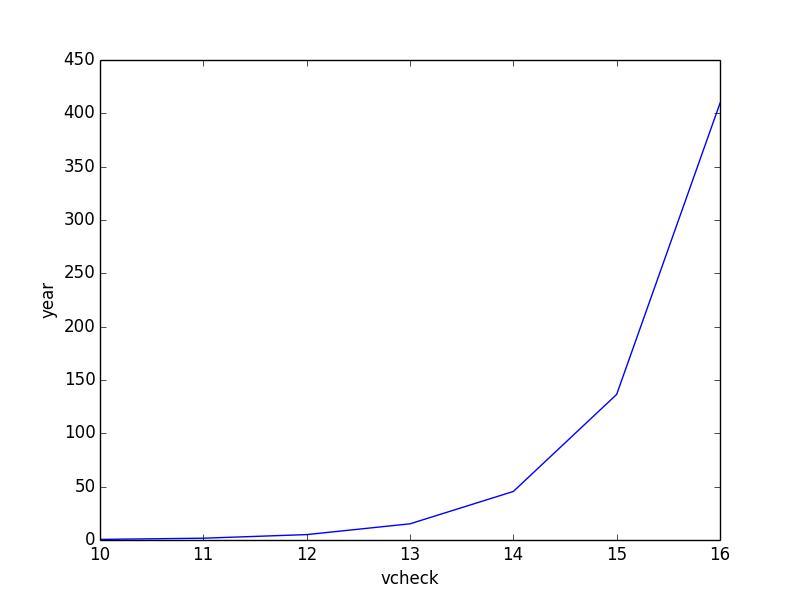
\includegraphics[width=10cm]{images/year.png}
	  \caption{It shows the waiting time for an adversary for a successful attack given that every parachain validators changes every 5 minutes}
	  \label{fig:totaltime}
\end{figure}

As it can be seen,  if $\totalchecks$ is more than 14, the adversary needs to wait more than 50 years for the attack. Therefore, in terms of security, it is important to have  minimum $\totalchecks$ validators.

\paragraph{The parameter $\mu$:} The possible $\mu$ (minimum number of extra check) values:

\begin{itemize}
    \item If $\mu = 0$, then $|pv| = 14$ in order to make sure that minimum $\totalchecks$ is always equal to $14$. Given that $|pv| = n/m$ where $m$ is the number of parachain validators $n = 14 * m$. 
    
    \item If $\mu > 0$, then $|pv| < 14$. It means that we need less validators for the security than in the case where $\mu = 0$. Less validators imply less network delay and less network delay implies more secure BABE. On the other hand, if $\mu$ increases, it means that more validators need to reconstruct a blob in order to check the validity. So, validators need to do more work. In terms of scalability of the relay chain, we need to decide $\mu$. 
\end{itemize}
As rule of thumb, if we don't care about the number of validators as far as it is not the maximum  number of validators ($N$) that Polkadot can handle, then if $14 * m < N$, $\mu = 0$. Otherwise, $\mu = 14 -N/m$. 

Another disadvantage of having $\mu = 0$ is that parachain validators have a less risky attack  when all of them are malicious. Imagine a parachain with a few collators. We can assume that they may be malicious and collaborate with the malicious validators. In this case, the validators will not have any report. So, there will be 0 extra checks. As soon as all parachain validators are malicious in this malicious parachain, they can add invalid block headers and cannot be caught. The security argument says here that they need to wait around 50 years for this, so the attack is not possible. However, in the real life, since the attack does not have any risk, the collators can bribe parachain validators with their stake and parachain validators validate an invalid blob.


Theorem \ref{thm:vcheckmal} gives the risk that  malicious validators take at  when they put an invalid report.  If $\mu + r \leq n/m$, the invalid block will not be detected with probability $\exp(-\frac{2}{3}(\mu+r))$. In the worst case scenario, if no report is received then the attack probability is $\exp(-\frac{2}{3}(\mu))$. We give in Figure \ref{fig:mu} that the probability of a successful attack in the case of $\totalchecks$ malicious validators are selected. As it can be seen in Figure \ref{fig:mu}, their risk is exponentially increasing when $\mu$ increases. In order to make the risk close to 0 even if no report received, $\mu$ should be greater than $4$.

\begin{figure}[h]\centering
	  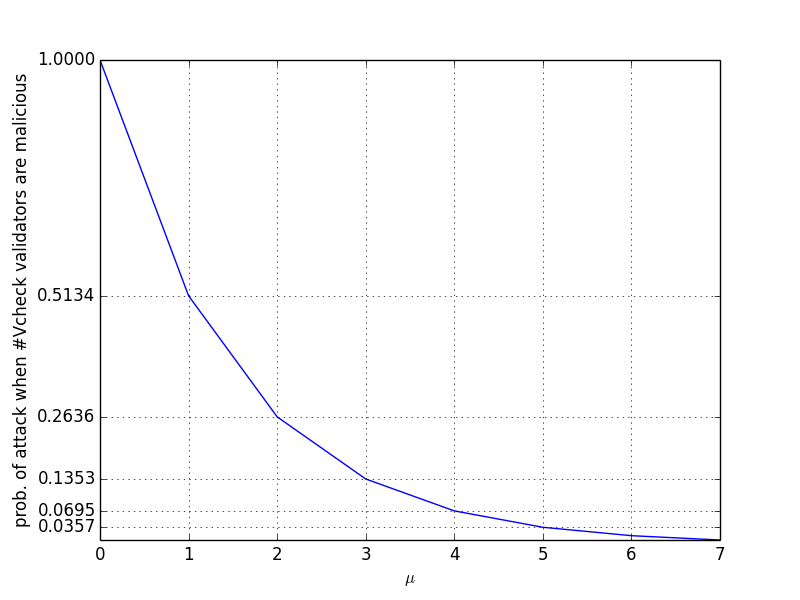
\includegraphics[width=12cm]{images/muval.png}
	  \caption{The risk of malicious validators when they attack even if $\totalchecks$ validators are malicious}
	  \label{fig:mu}
\end{figure}

\paragraph{Fisherman and Collator Reports:} In the validity scheme, we rely on the invalidity reports of fishermen and unavailability reports of collators to find the parameter $ \totalchecks $. However, we need to bound $\totalchecks$ so that these reports do not make too many validators check the validity. Let us call this bound $\mu_{max}$ (i.e, $\mu + \lceil r_f + r_a \rceil \leq \mu_{max}$). This bound is necessary because regular malicious reports can slow down the process easily. 

When a fisherman sends a report of invalidity, but later on it is found to be valid, the fisherman is slashed. Therefore, the reliability of a fisherman report can be measured by how much it is staked. 
Considering this, $r_f$ can be computed as follows:

$$r_f = \frac{\sum_{i}\mathsf{stake}_{f_i}}{v_{gain}}$$

Here, $\mathsf{stake}_{f_i}$ is the stake that a fisherman $f_i$ puts for this report and $v_{gain}$ is the DOT value that a validator receives in each block. In a nutshell, a fisherman needs to stake at least the same amount that the validator earns for each block in order to make a validator to execute an extra validity check. If the fisherman report is not valid, then the fisherman pays for this extra check. So, a malicious fisherman has to spend $\mu_{max} v_{gain}$ for a report to slow down the validator network. We believe that this model discourages fishermen from sending false reports. 

However, we cannot measure the reliability of unavailability reports as fisherman's reports since it is not possible to show the correctness or incorrectness of any unavailability reports. Malicious collators do not lose anything by just sending fake unavailability reports. In order to solve this issue, we assign a parameter $\alpha \in (0,1)$ for a parachain that defines the proportion of honest collator assumption. Depending on $\alpha$, we have defined $r_a$ for two cases:
\begin{itemize}
    \item if $\alpha > 1/2$, $r_a = \mu_{max}^{x/\alpha}$ 
    
        \[   
    r_a(x)= 
     \begin{cases}
       \mu_{max}^{x/\alpha} & \text{if } x \leq \alpha \\
       \mu_{max} &\text{otherwise} \\ 
     \end{cases}
\]  
    
    where 
    $$x = \frac{\text{total unavailability reports}}{\text{all collators}} = \frac{\sum_{c_i \in C_P}st_{c_i}}{|C_P|}.$$
    
    Here, $st_{c_i}\in \{0,1\}$ and it is 0 if the block is available. Otherwise, it is 1. The reason of using a function such as $\mu_{max}^{x/\alpha}$ is to make sure that we have extra checks close to maximum check only if the number of unavailability reports are close to the number of honest collator assumption. Thanks to this, if the number of honest collators are majority, the malicious collators who want to slow down Polkadot cannot achieve to make always maximum number of checks with only unavailability reports. In general, these type of parachains can be investigated by fishermen as far as the blocks are available to honest collators. Therefore, we expect that if there is any invalid block, the fishermen catch it and send a report. If the blocks are unavailable to honest collators (so fishermen too), validators check the invalidity with the maximum capacity.  
    
    \item if $\alpha < 1/2$, then it is critical to give more importance to the unavailability reports from this parachain. Therefore, we use the following linear function:
    
    \[   
    r_a(x)= 
     \begin{cases}
       \mu_{max}\frac{x}{\alpha} & \text{if } x \leq \alpha \\
       \mu_{max} &\text{otherwise} \\ 
     \end{cases}
\]  
\end{itemize}

So, $\mu' = \mu + \lceil r_a + r_f \rceil$ if $\mu + \lceil r_a + r_f \rceil \leq \mu_{max}$. Otherwise, $\mu' = \mu_{max}$.


\paragraph{The parameter $\mu_{max}$:} Given the fact that we have maximum number of extra checks when there are many invalidity or unavailability  reports, the parameter $\mu_{max}$ needs to be big enough so that the probability of having at least one honest extra check is almost 1.
This probability can be bounded by $1-(\frac{1}{3})^{\mu_{max}}$. Therefore, we can have $\mu_{max} = 15$.

In Figure \ref{fig:ra}, we compute the number of extra checks required depending on the $\alpha$-parameter of a parachain. As it can be seen, the parachain that we trust less requires more extra-checks. The parachain where we assume honest majority reaches the maximum check when the unavailability reports are close to the number of honest collators.  


\begin{figure}[h]\centering
	  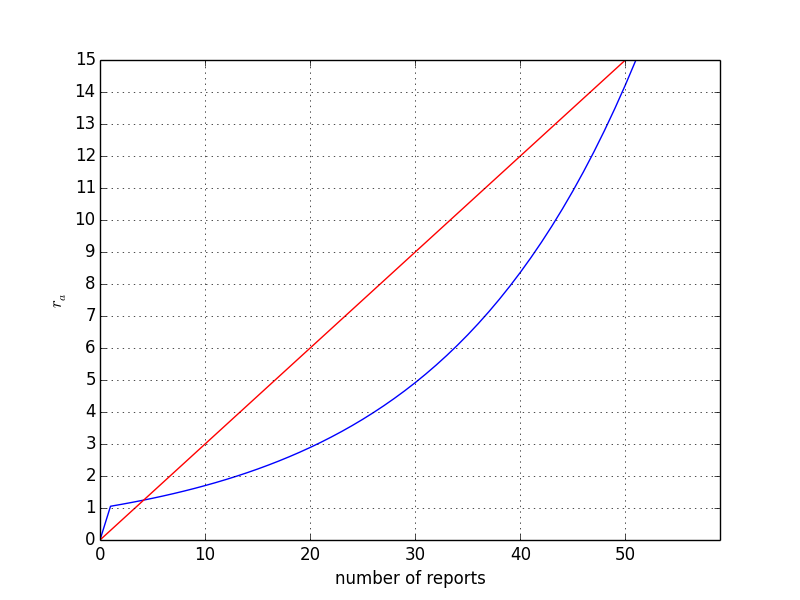
\includegraphics[width=10cm]{images/ra.png}
	  \caption{The red and blue graph shows the number of required extra checks when $\alpha \leq 1/2$ and $\alpha > 1/2$. Here, we assume that the total number of collators are 100.}
	  \label{fig:ra}
\end{figure}



\appendix
\section{Proof Details}

\newcommand\valord{\ensuremath{\mathcal{O}}}

\begin{lemma}\label{lem:permutation}
For any slot number $s$, block producer $bp$, epoch randomness $r$ for the epoch that includes $s$, integer $k >0$, and parachain $P$, with probability at least $1-(f/n)^{-k}$ over the epoch randomness and the random oracles for the hashes and VRFs, for any block that $bp$ produces in slot $s$ that includes a parachain header from $P$, if we eventually have $\totalchecks \geq k$ for this parachain header, then some honest validator checks the parachain block.
\end{lemma}
\begin{proof}
Consider generating an ordering $\valord$ of validators as follows, first we have the parachain validators in a uniformly random order, then all validators who satisfy condition (\ref{cond:mod}) (using $bp$'s VRF for slot $s$) in a uniformly random order, then we order all remaining validators in increasing order of the hash $H(ID_{PC} || \mathtt{VRF}_{\sk^v_j}(V))$ used in condition (\ref{cond:time}), breaking ties due to collisions in a uniformly random order. We claim that distribution of $\valord$ is as a uniformly random permutation of the validator set. To see this note that the only operation for which the different validators are treated differently are the VRFs and we assume that they are random oracles. The parachain validators are a set of $n/m$ validators chosen uniformly at random using $r$. Each validator satisfies condition (\ref{cond:mod}) with the same probability independently and so the distribution of the set of validators satisfying (1) conditioned on its size is a set of that size chosen uniformly at random from the non-parachain validators. Also the hashes in (2) are independently and identically distributed.

Next we show that for any block $bp$ produces in slot $s$ which includes a parachain header for $P$,  if any honest validator ever sees that $\totalchecks \geq k$, then any honest validators in the first $k$  validators in $\valord$ eventually check that block. All honest parachain validators and honest validators who satisfy (\ref{cond:mod}) check. If all honest validators in the fist $k$ validators in $\valord$ satisfy these conditions we are done. So suppose that $v$ is an honest validator in the first $k$ validators in $\valord$ who doesn't satisfy either of these conditions. $v$ will still check if $\tau$ is large enough and they don't see attestation from $\totalchecks$ validators who either are parachain validators, satisfied condition (\ref{cond:mod})  or had a smaller hash in condition (\ref{cond:time}). But noting that all such validators are before $v$ in $\valord$ so there can be at most $k-1$ of them. Thus $v$ only ever counts $k-1$ attestations towards the number needed $\totalchecks$ which is eventually $\geq k$. So when $\totalchecks \geq k$ and $\tau$ is large enough, $v$ checks.

Finally we need to show that the probability that the first $k$ validators in $\valord$ are honest is at least $(f/n)^k$. Since the first $k$ validators in $\valord$ are distributed as a set of $k$ validators chosen uniformly at random, this probability is $\prod_{i=0}^{k-1} (f-i)/(n-i) \leq (f/n)^k$.
\end{proof}

\end{document}
